\documentclass[12pt,]{article}
\usepackage[utf8]{inputenc}
\usepackage[T1]{fontenc}
\usepackage{mathptmx}
\usepackage{geometry}
\usepackage{mathtools}
\usepackage[english]{babel}
\usepackage{graphicx}
\usepackage[os=win]{menukeys}
\usepackage[figurename=Gambar]{caption}
\usepackage{hyperref}
\usepackage{minted}

\newcommand{\WindowsLogo}{\raisebox{-0.1em}{
\includegraphics[height=0.8em]{winlogo/Windows_3_logo_simplified}}}
\newcommand{\PowerLogo}{\raisebox{-0.1em}{
\includegraphics[height=0.8em]{winlogo/power}}}
\newcommand{\WinKey}{\keys{\WindowsLogo}}	
\newcommand{\PowerKey}{\keys{\PowerLogo}}	

\addto\captionsenglish{\renewcommand{\contentsname}{Daftar Isi}}

\hypersetup{
	colorlinks=true, %set true if you want colored links
	linktoc=all,     %set to all if you want both sections and subsections linked
	linkcolor=blue,  %choose some color if you want links to stand out
}

\geometry{
	a4paper,
	left=15mm,
	right=10mm,
	top=10mm,
	bottom=10mm,
}

\title{\Large \bf
Tutorial Penggunaan AchmadiOS
}

\author{Achmadi ST}

\date{}

\begin{document}
	
	\maketitle
	\thispagestyle{empty}
	\pagestyle{empty}
	
	\begin{figure}[h]
		\centering
		
\includegraphics[width=300pt]{archlinuxlogo.png}
	\end{figure}

	\newpage
	(catatan: Daftar Isi dan Index bisa diklik)
	\tableofcontents
	
	\newpage
	\section{Perkenalan}

	Saat ini telah tersedia beragam varian sistem operasi GNU/Linux untuk beragam kebutuhan.
	Diantara sekian banyak sistem operasi, semuanya memiliki kelebihan masing-masing.
	Disini penulis memilih salah satu distro yang dikenal sangat flexibel dan sangat dekat dengan upstream, yaitu Arch Linux.
	Poin penting kelebihan Arch Linux dijelaskan sebagai berikut:

	\begin{itemize}
		\item Flexibilitas. Arch Linux sangat flexibel karena pada dasarnya user sendiri yang menentukan paket apa saja yang dibutuhkan dan yang diinstal
		\item Upstream. Arch Linux sebagai sebuah distribusi, mengambil apa-adanya dari projek-projek upstream sesegera mungkin dengan patch sesedikit mungkin.
	\end{itemize}

	Akan tetapi, mengingat user yang menentukan dan membangun sendiri, Arch Linux sering tidak direkomendasikan untuk pengguna GNU/Linux pemula.
	Sifat DIY (Do It Yourself) ini sering membuat pengguna pemula ragu untuk mencobanya.
	Dengan alasan tersebut, penulis hadirkan AchmadiOS, sebuah distro berbasis Arch Linux langsung dari repository resmi Arch Linux.

	Selain AchmadiOS, sebenarnya ada distro lain yang juga merupakan turunan Arch Linux.
	Sebut saja Manjaro, namun disini Manjaro menggunakan repository binary terpisah dengan Arch Linux.
	Kemudian semisal Antergos, namun rumor yang beredar Antergos tetap membutuhkan koneksi untuk instalasi.
	
	\begin{figure}[h]
		\centering
		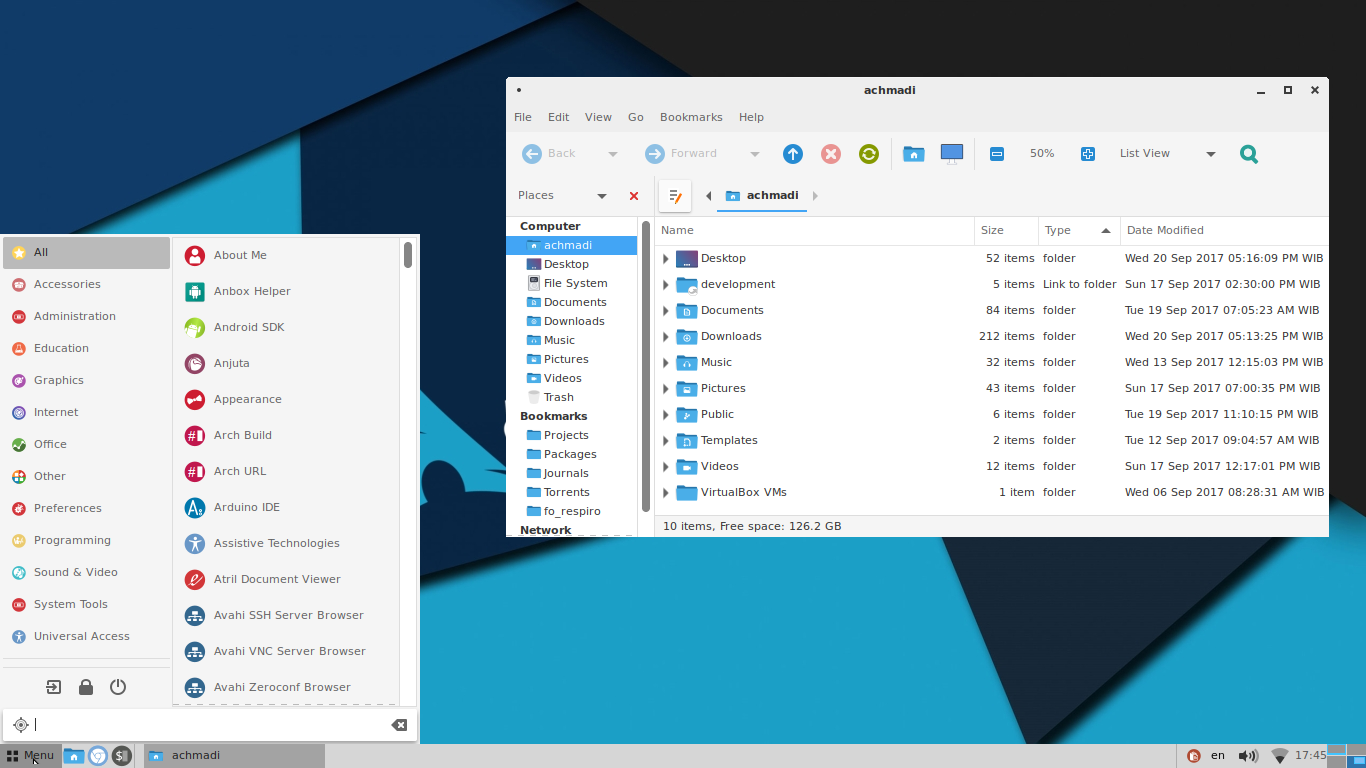
\includegraphics[width=250pt]{png/tema_1}
		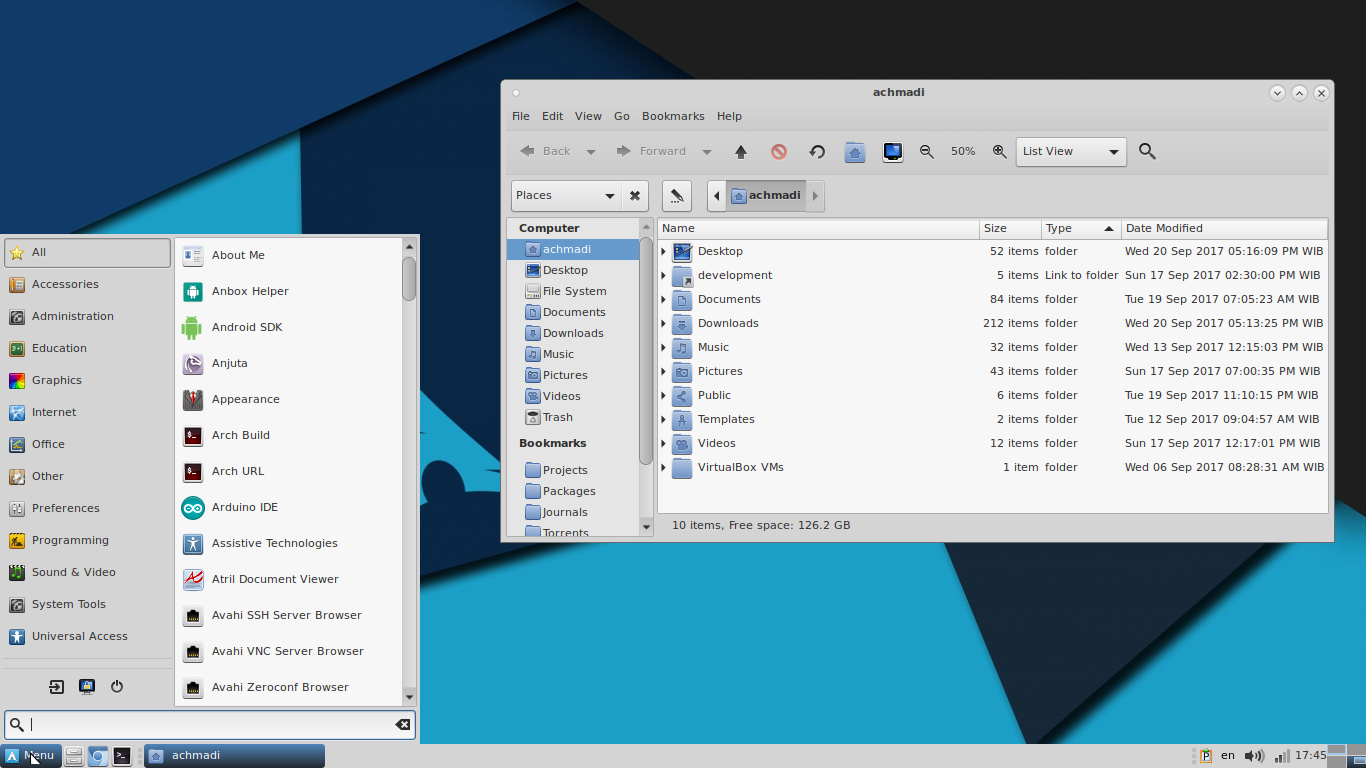
\includegraphics[width=250pt]{png/tema_2}
		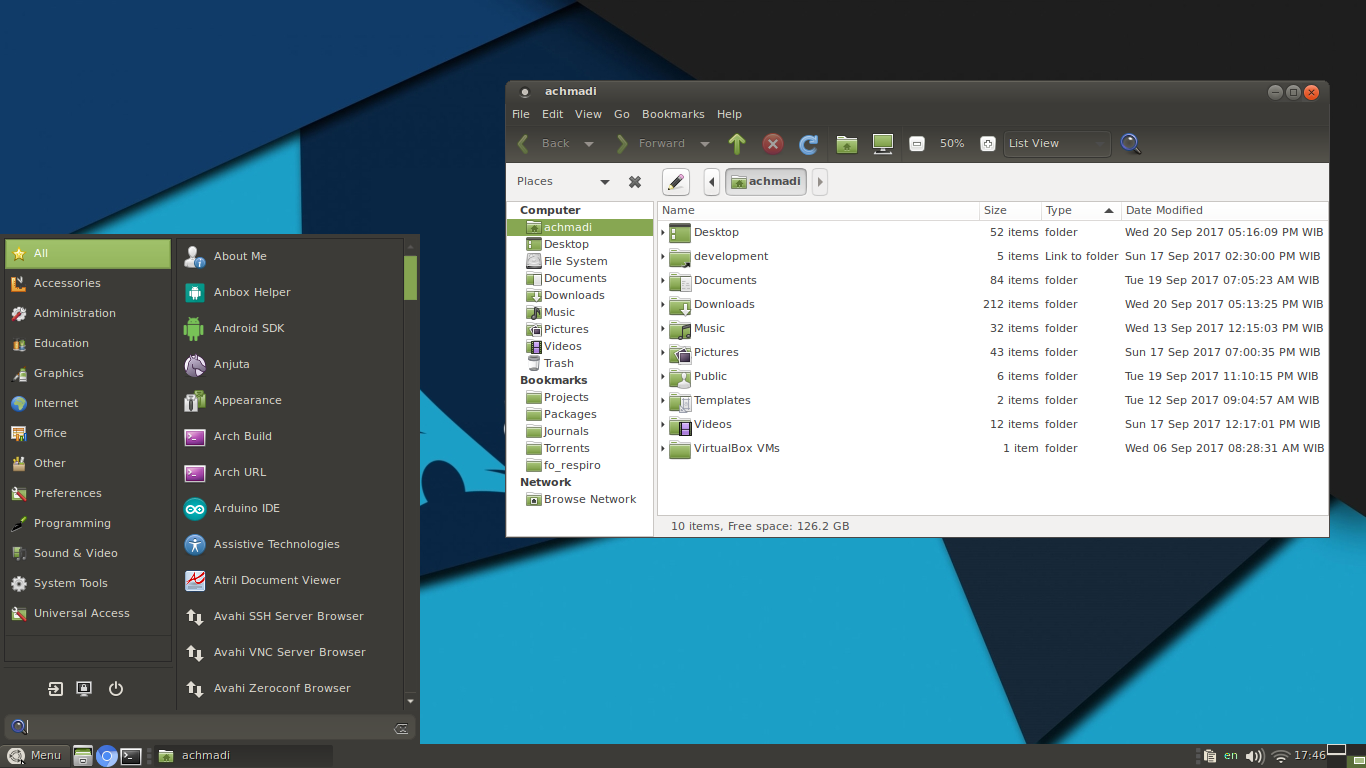
\includegraphics[width=250pt]{png/tema_3}
		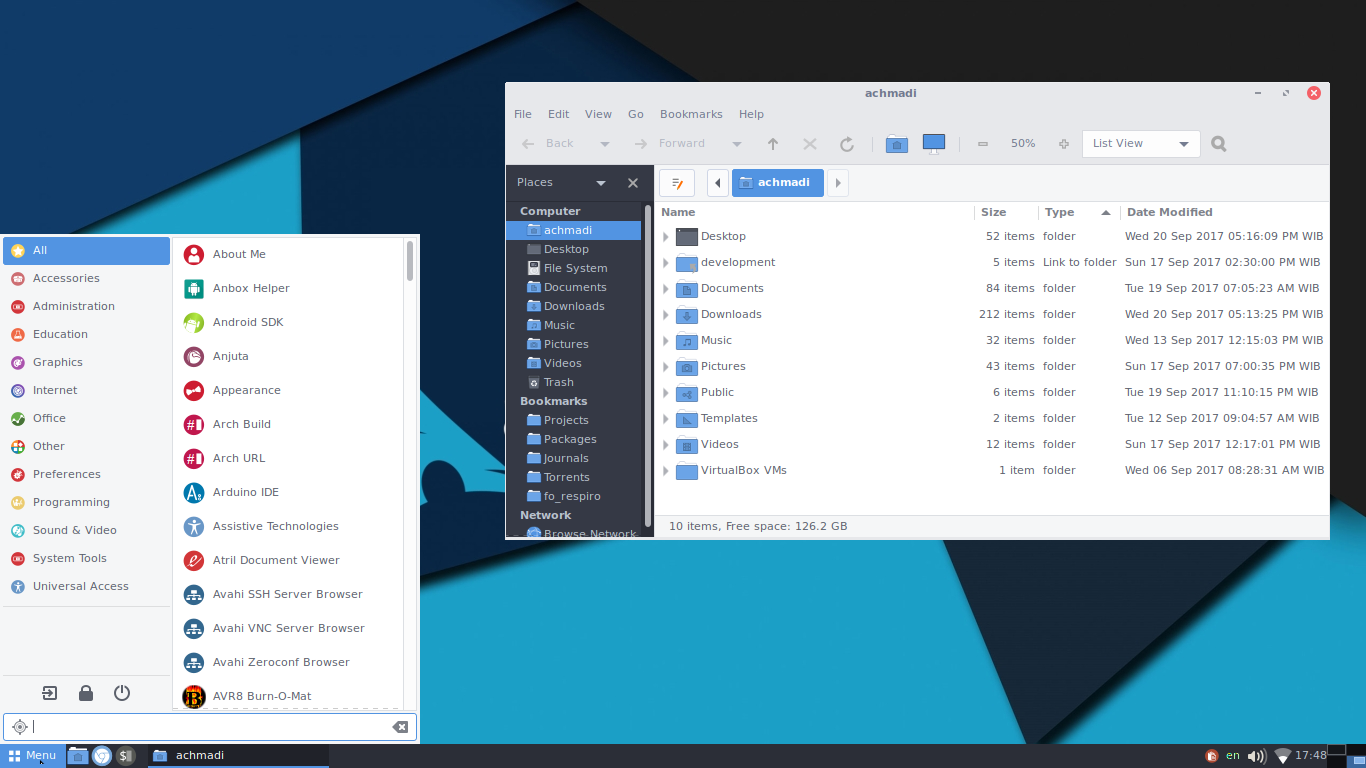
\includegraphics[width=250pt]{png/tema_4}
		\caption{Desktop AchmadiOS dalam 4 tema berbeda}
	\end{figure}

	\newpage

	\section{Start-up}

	Berikut akan dijelaskan penggunaan AchmadiOS yang telah terinstal dalam sebuah PC/Laptop.

	\subsection{Booting}

	Saat pertama booting, maka akan muncul tampilan GRUB sebagaimana gambar berikut:

	\begin{figure}[h]
		\centering
		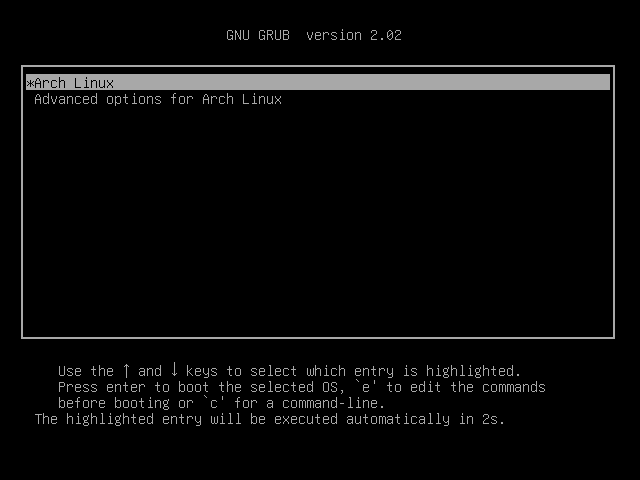
\includegraphics[width=300pt]{png/grub}
		\caption{Tampilan GRUB menu}
	\end{figure}

	Pada tampilan grub tersebut, juga akan ada pilihan OS lain semisal Windows apabila terinstal bersama AchmadiOS (dual-boot).
	Untuk memilih gunakan tombol panah atas ($\uparrow$) dan bawah ($\downarrow$) pada keyboard.
	Selanjutnya tekan tombol Enter (\keys{\return}) untuk memilih mana yang akan diboot.
	Default timeout untuk memilih adalah 5 detik.
	Setelah menekan Enter, maka AchmadiOS akan mulai booting sebagaimana gambar dibawah:

	\begin{figure}[h]
		\centering
		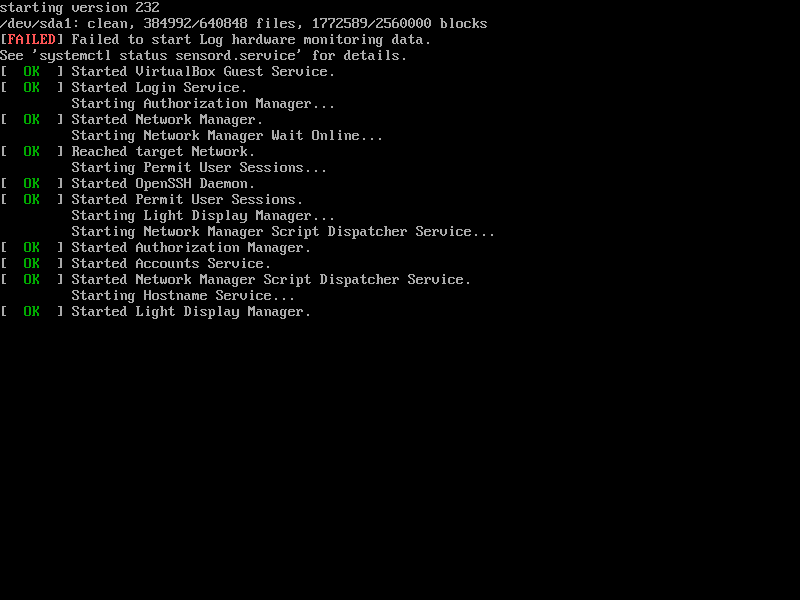
\includegraphics[width=300pt]{png/boot}
		\caption{Tampilan proses booting}
	\end{figure}

	Tunggu beberapa saat maka proses booting akan selesai. Pada tahap ini kemungkinan selanjutnya ada dua:

	\begin{itemize}
		\item Masuk Login Manager. Akan dijelaskan di sub-bab selanjutnya.
		\item Masuk Desktop. Pada tahap ini sudah siap dipakai.
	\end{itemize}

	\newpage

	\subsection{Login Manager}

	Setelah proses booting, maka apabila belum di atur autologin, maka yang masuk adalah tampilan login manager sebagaimana berikut:

	\begin{figure}[h]
		\centering
		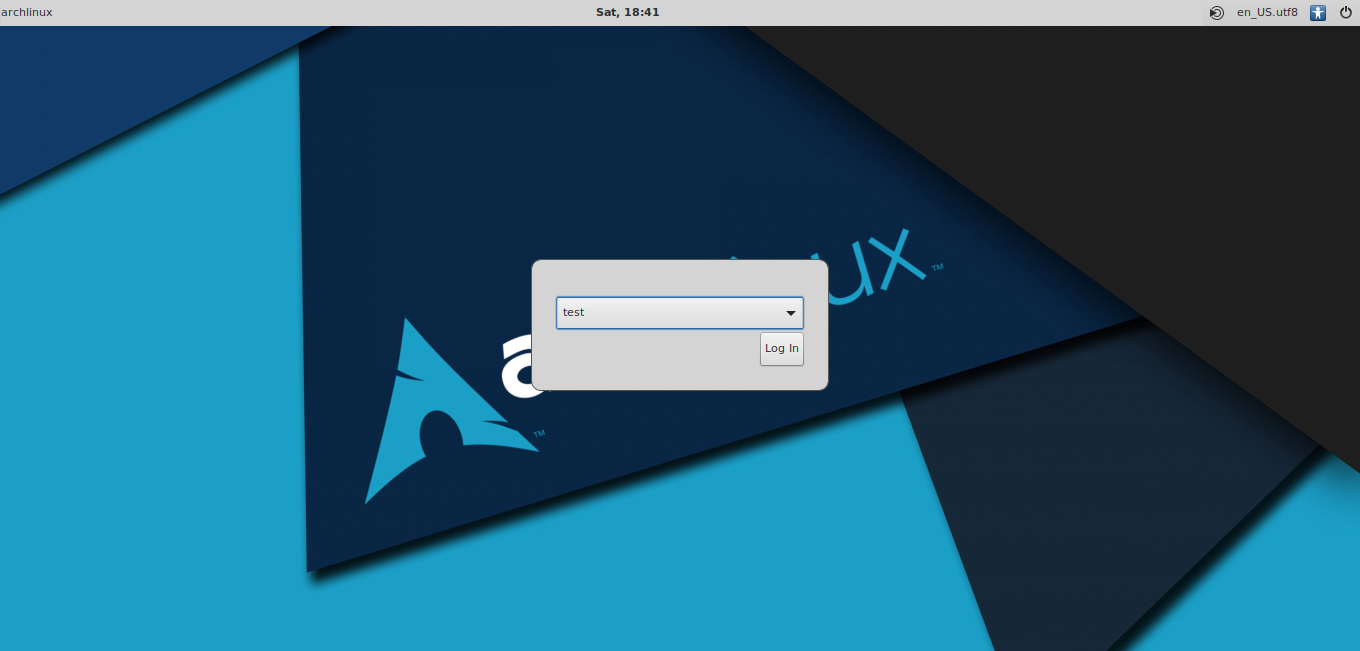
\includegraphics[width=300pt]{png/login}
		\caption{Tampilan Login Manager}
	\end{figure}

	Anda dapat memilih user yang akan menjadi ID anda untuk masuk.
	Anda juga dapat memilih bahasa yang dipakai dengan memilih pilihan bahasa yang ada di pojok kanan atas.

	\begin{figure}[h]
		\centering
		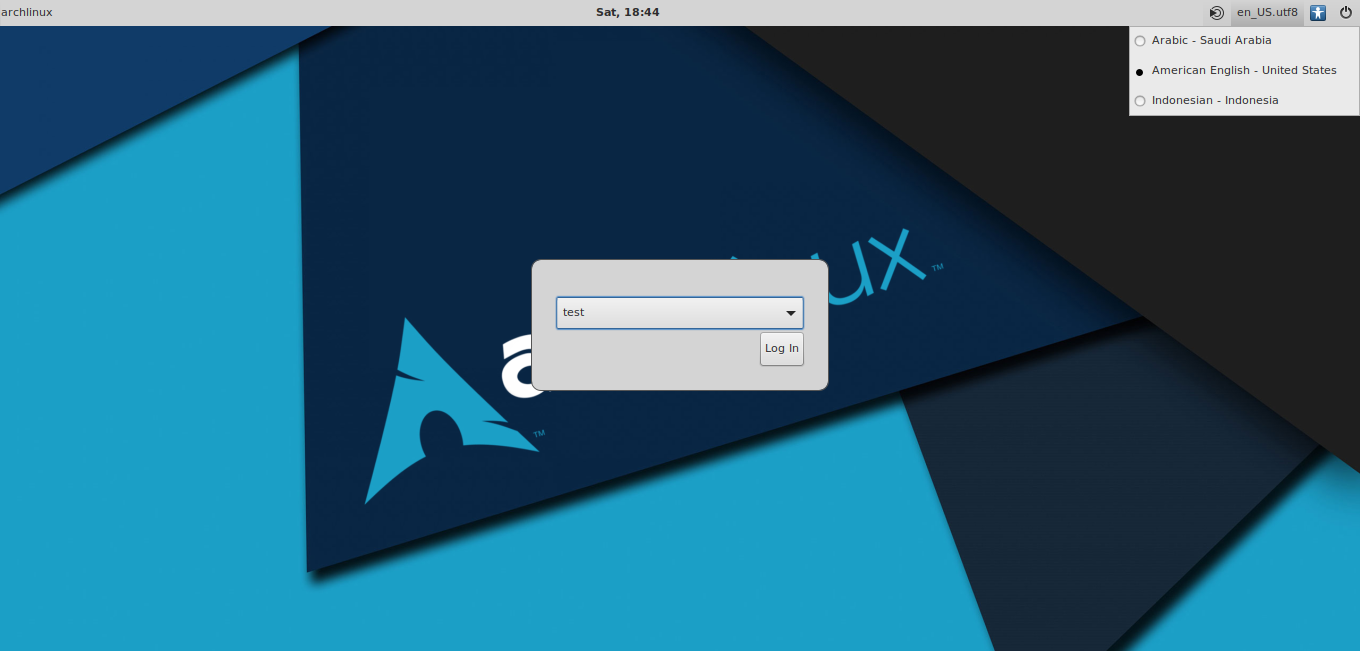
\includegraphics[width=300pt]{png/login_lang}
		\caption{Tampilan Pilihan Bahasa}
	\end{figure}

	Sebagaimana terlihat, pilihan bahasa yang telah tersedia adalah:

	\begin{itemize}
		\item Arabic (Saudi Arabia)
		\item American English (United States)
		\item Indonesian (Indonesia)
	\end{itemize}

	Setelah memilih apa yang diinginkan, untuk masuk tinggal klik \textbf{Log In} atau tekan tombol Enter (\keys{\return}) pada keyboard.
	Tunggu beberapa saat maka anda akan masuk desktop.

	\newpage

	\section{Desktop}

	Berikut adalah tampilan dasar desktop yang dirancang mirip dengan tampilan Windows 7.

	\begin{figure}[h]
		\centering
		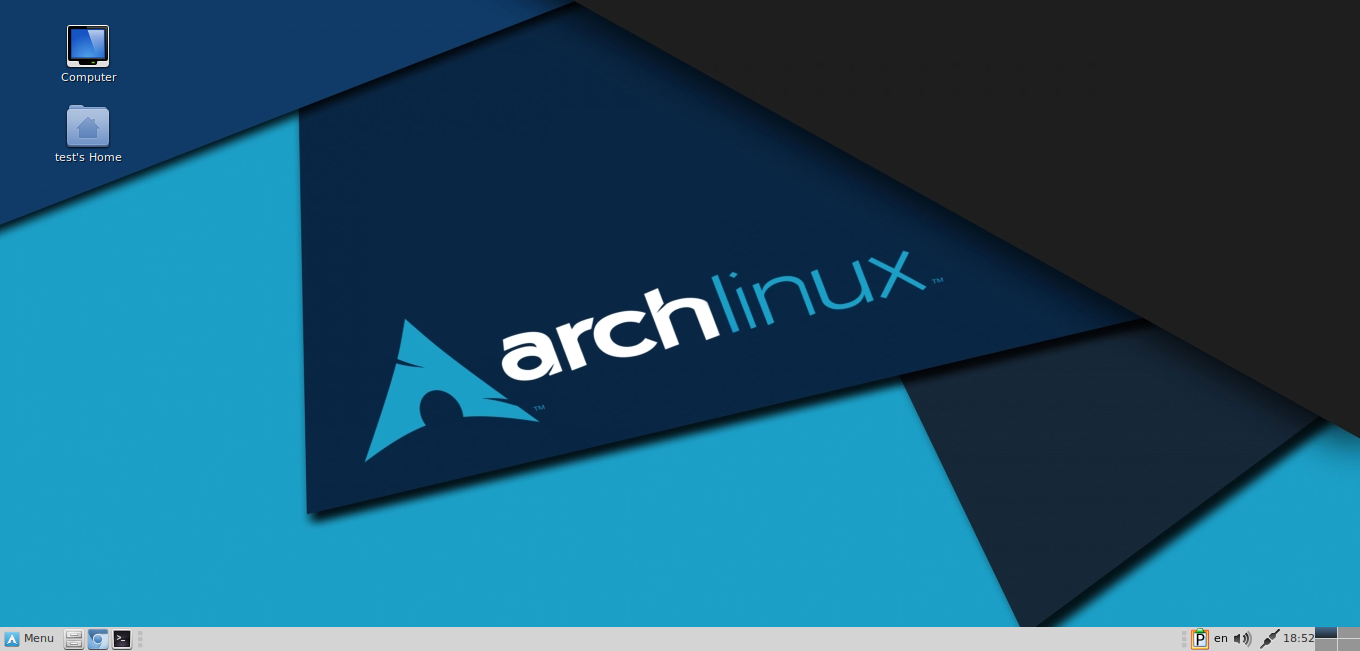
\includegraphics[width=300pt]{png/desktop}
		\caption{Tampilan Desktop}
	\end{figure}

	Adapun bagian-bagiannya adalah sebagai berikut:

	\begin{figure}[h]
		\centering
		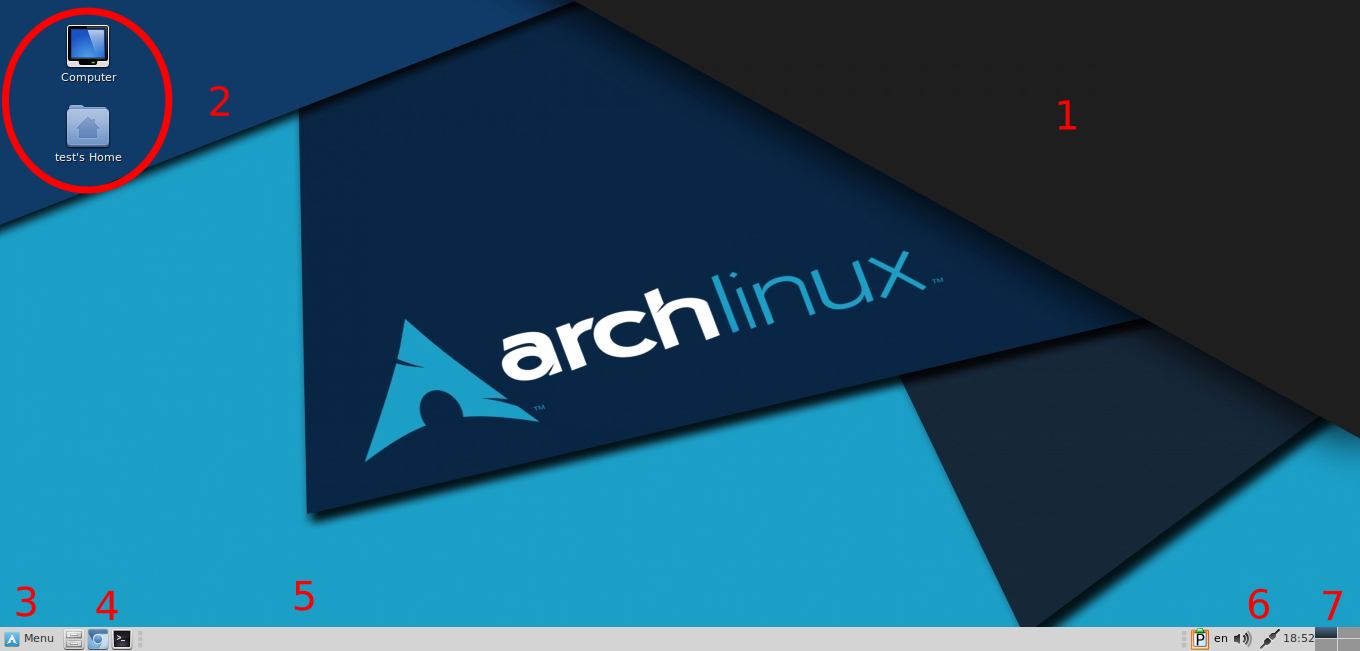
\includegraphics[width=300pt]{png/desktop_part}
		\caption{Bagian-bagian Desktop}
	\end{figure}

	\begin{enumerate}
		\item Desktop. Anda dapat menaruh berkas(file) atau directory (folder) disini
		\item Directory ke Computer dan Home
		\item Menu. Anda dapat memanggil program dari sini
		\item Program shortcut. Anda dapat menaruh dan memanggil program favorit anda dari sini
		\item Panel Window List. Program yang berjalan akan tampil disini layaknya Taskbar di Windows
		\item System Tray. Disini terdapat systray untuk pengaturan Audio, Wifi/LAN, Jam, Batere, dst.
		\item Workspace List. Disini anda dapat berpindah dari satu workspace (virtual desktop) ke workspace lain.(catatan: Fitur ini baru ada pada Windows 10).
	\end{enumerate}

	\newpage

	\section{Menu}

	Berikut bagian penting dari desktop adalah menu yang berada pada pojok kiri bawah.
	Anda dapat mengaksesnya dengan klik mouse atau tombol Windows (\WinKey)

	\begin{figure}[h]
		\centering
		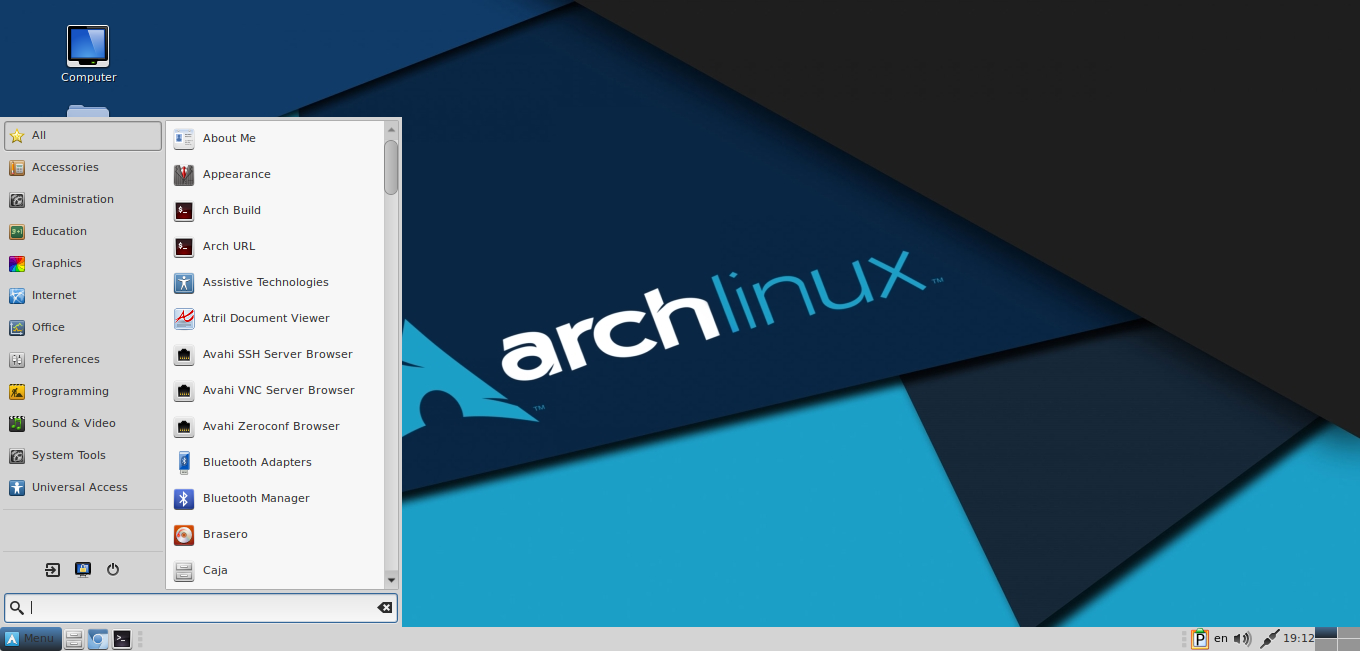
\includegraphics[width=300pt]{png/menu}
		\caption{Tampilan Menu}
	\end{figure}

	Adapun bagian-bagiannya adalah sebagai berikut:

	\begin{figure}[h]
		\centering
		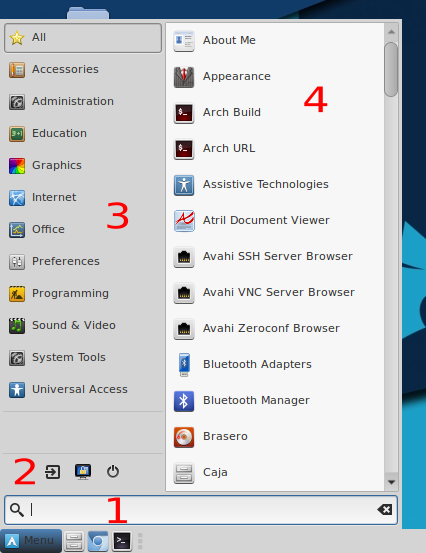
\includegraphics[width=250pt]{png/menu_part}
		\caption{Bagian utama Menu}
	\end{figure}

	\begin{enumerate}
		\item Search Area. Anda dapat memasukkan sebagian nama dari program yang anda cari
		\item Session Control. Secara berurutan dari kiri Logout, Lock, dan Shutdown/Restart/Suspend
		\item Kategori untuk mempermudah pencarian menu
		\item Menu program yang bisa dijalankan
	\end{enumerate}

	\newpage

	\section{Session Control}

	Selanjutnya adalah petunjukan kendali sesi, baik itu Shutdown/Restart/Suspend, Lock, atau Logout.
	Perlu diingat bahwa disebabkan sekian banyak problem yang mengikuti partisi SWAP, maka penulis sengaja tidak menyediakan fitur Hibernate.

	\subsection{Shutdown/Restart/Suspend dari Menu}

	Aksi mematikan komputer memiliki pilihan sebagai berikut
	\begin{itemize}
		\item Shutdown. Yaitu aksi mematikan komputer.
		\item Restart. Yaitu Shutdown namun dilanjutkan dihidupkan kembali.
		\item Suspend. Yaitu menonaktifkan sebagian besar sistem. Istilahnya sama dengan Sleep
	\end{itemize}
	
	Untuk melakukan Shutdown/Restart, klik \textbf{Menu} dan selanjutnya klik \textbf{Turn off the device} (yang dilingkari merah)

	\begin{figure}[h]
		\centering
		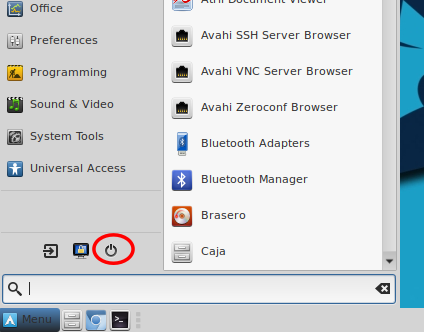
\includegraphics[width=300pt]{png/turnoff}
		\caption{Tombol menu matikan}
	\end{figure}

	Maka akan muncul dialog seperti ini:

	\begin{figure}[h]
		\centering
		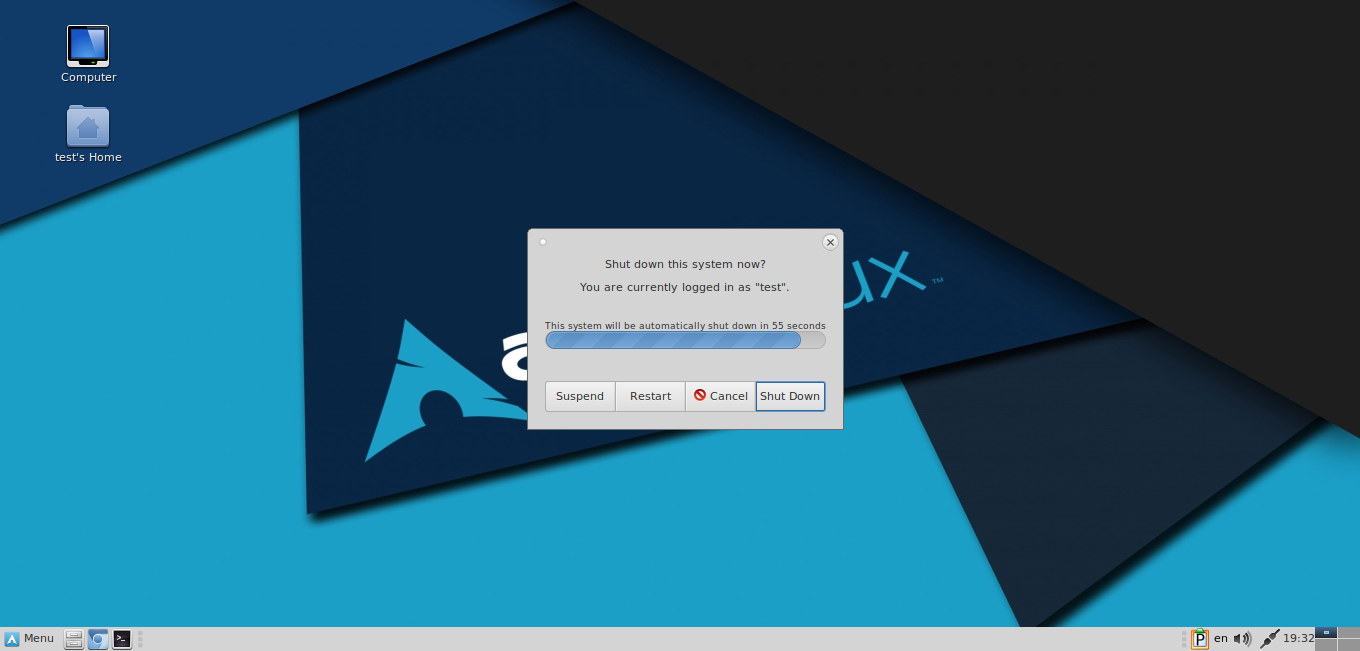
\includegraphics[width=300pt]{png/turnoffdlg}
		\caption{Dialog Matikan}
	\end{figure}

	Pilihan yang tersedia adalah \textbf{Shut Down}, \textbf{Restart}, \textbf{Suspend} (atau Sleep), dan \textbf{Cancel}.
	Jika tidak ada aksi dari pengguna selama 60 detik, maka otomatis perintah Shut Down akan dijalankan.

	\newpage

	\subsection{Shutdown/Restart/Suspend dari Login Manager}

	Untuk melakukan Shutdown/Restart dari Login Manager, klik tombol Power (\PowerKey) di pojok kanan atas (dilingkari merah)

	\begin{figure}[h]
		\centering
		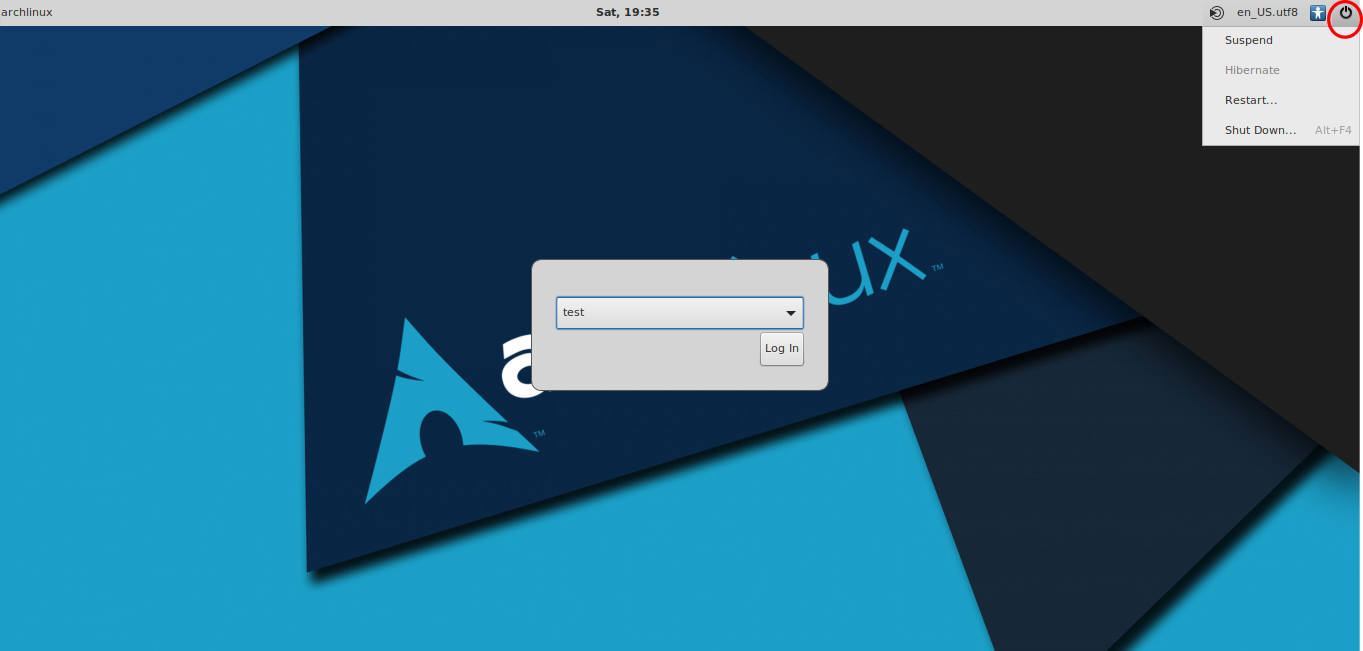
\includegraphics[width=300pt]{png/turnofflogman}
		\caption{Tombol pilihan matikan pada Login Manager}
	\end{figure}

	Pilihan yang tersedia adalah  \textbf{Shut Down}, \textbf{Restart}, \textbf{Suspend} (atau Sleep), dan Hibernate.
	Namun pilihan Hibernate disini tidak bisa dipilih karena memang tidak disediakan.

	\newpage

	\subsection{Logout dari Menu}

	Logout disini adalah kendali sesi untuk mengakhiri sesi yang sedang berjalan, baik untuk ganti ID user atau memang diperlukan suatu aksi re-login.
	Untuk Logout, klik \textbf{Menu} dan selanjutnya klik \textbf{End the Current Session}

	\begin{figure}[h]
		\centering
		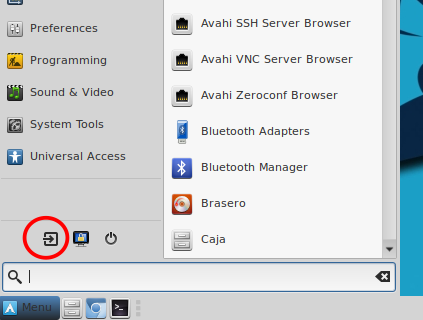
\includegraphics[width=300pt]{png/logout}
		\caption{Tombol pilihan Logout}
	\end{figure}

	Maka akan muncul dialog seperti ini:

	\begin{figure}[h]
		\centering
		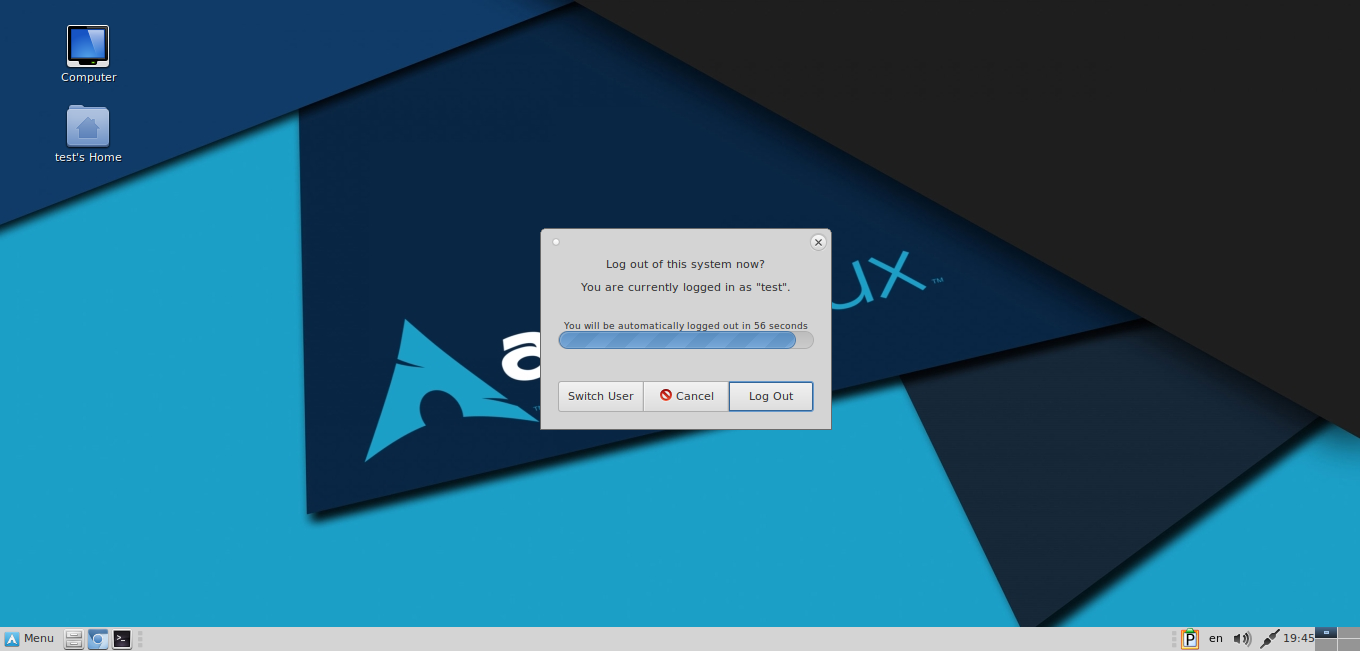
\includegraphics[width=300pt]{png/logoutdlg}
		\caption{Dialog Logout}
	\end{figure}

	Pilihan yang tersedia adalah \textbf{Switch User}, \textbf{Cancel}, dan \textbf{Log Out}.
	Perbedaan Switch User dengan Log Out adalah Switch User dapat digunakan berpindah ke user lain tanpa harus benar-benar mengakhiri sesi yang sekarang.
	Jika tidak ada aksi dari pengguna selama 60 detik, maka otomatis perintah Log Out akan dijalankan.

	\newpage

	\subsection{Lock dari Menu}

	Lock disini maksudnya adalah mengunci layar tanpa ada aksi terhadap sesi yang sedang berjalan.
	Untuk Lock, klik \textbf{Menu} dan selanjutnya klik \textbf{Lock the Screen}

	\begin{figure}[h]
		\centering
		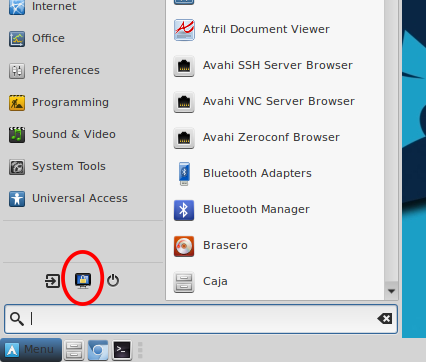
\includegraphics[width=300pt]{png/lock}
		\caption{Tombol Lock}
	\end{figure}

	Maka setelah ditekan otomatis layar akan hitam dan terkunci.

	\newpage

	\section{Penggunaan Dasar}

	Berikut akan dijelaskan penggunaan dasar AchmadiOS

	\subsection{Explorer (Pengolah File)}

	Sebagai program yang berfungsi layaknya Explorer (Windows) disini adalah Caja.
	Anda dapat mengaksesnya dengan beberapa cara, misalnya:

	\begin{enumerate}
		\item Double Click Icon Computer atau Home di desktop.
		\item Shortcut Caja di panel
		\item melalui klik \textbf{Menu}, kemudian \textbf{System Tools}, kemudian \textbf{Caja} 
		\begin{figure}[h]
			\centering
			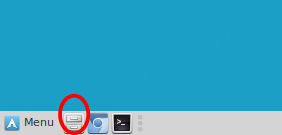
\includegraphics[width=200pt]{png/panelcaja}
			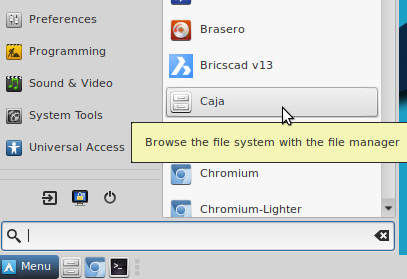
\includegraphics[width=200pt]{png/menucaja}
		\end{figure}
	\end{enumerate}

	Selanjutnya akan tampil jendela pengolah berkas (File Manager) layaknya Explorer di Windows.
	Anda dapat melakukan pengolahan berkas sebagaimana yang biasa anda lakukan di Explorer di Windows.
	Anda juga dapat mengakses data di drive yang dimiliki Windows melalui program ini.
	\begin{figure}[h]
		\centering
		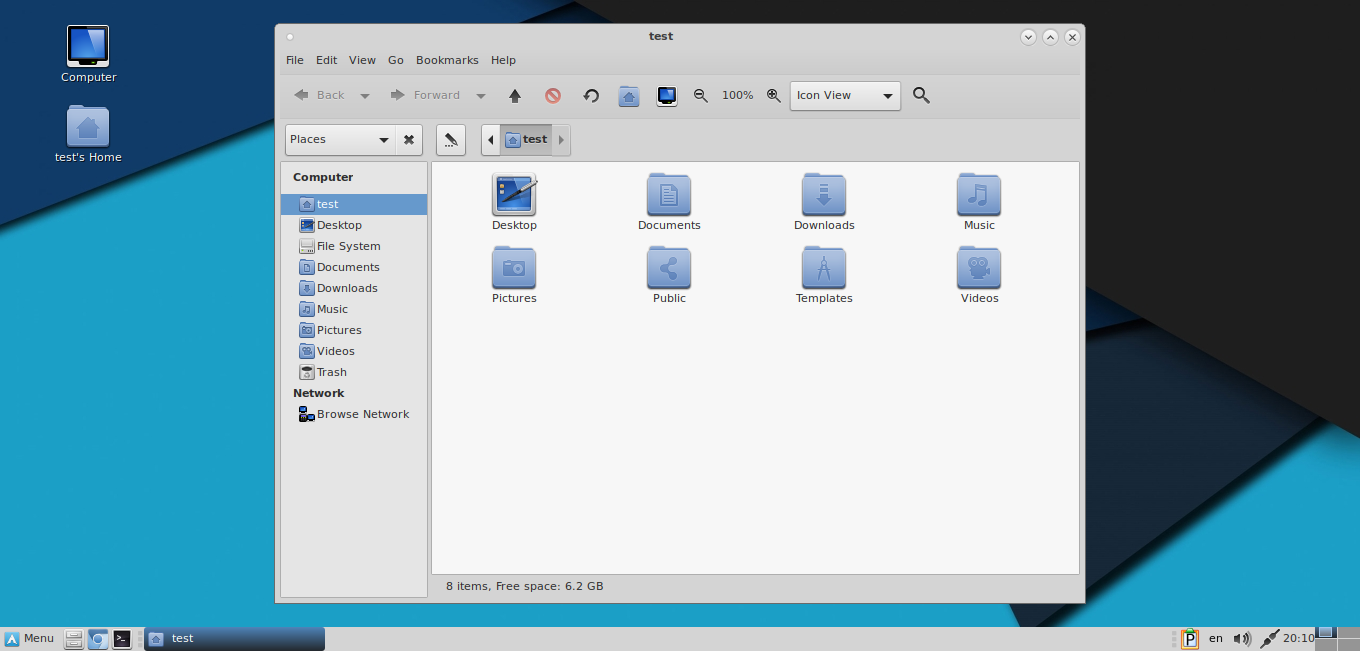
\includegraphics[width=300pt]{png/caja}
		\caption{File Manager Caja}
	\end{figure}

	\newpage

	\subsection{Web-browsing}

	Untuk melakukan perambanan internet (web-browsing), anda dapat menjalan program Chromium.
	Chromium adalah browser yang menjadi dasar program Google-Chrome.

	Anda dapat mengaksesnya dengan beberapa cara, misalnya:

	\begin{enumerate}
		\item Shortcut Chromium di panel
		\item melalui klik \textbf{Menu}, kemudian \textbf{Internet}, kemudian \textbf{Chromium} 
		\begin{figure}[h]
			\centering
			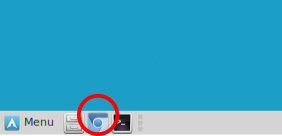
\includegraphics[width=200pt]{png/panelchromium}
			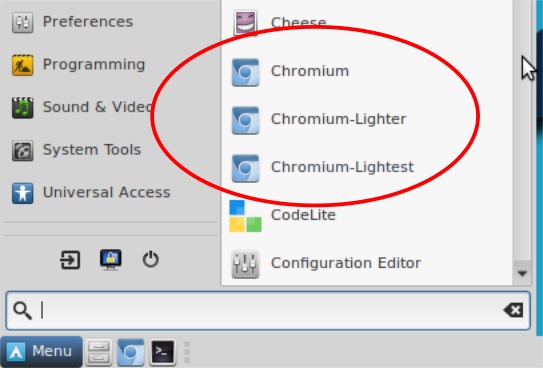
\includegraphics[width=200pt]{png/menuchromium}
		\end{figure}
	\end{enumerate}

	Catatan: Disini penulis sediakan Chromium yang dapat berjalan dalam 3 mode
	\begin{enumerate}
		\item Chromium. Mode Normal dimana berjalan apa adanya
		\item Chromium-Lighter. Mode single process. Disini semua proses tab berada dalam satu thread proses. Extension berada dalam satu proses lain. Dengan ini diharapakan memakan RAM lebih kecil.
		\item Chromium-Lightest. Sama dengan Chromium-Lighter namun seluruh Extension dimatikan.Dengan ini diharapakan memakan RAM paling kecil.
	\end{enumerate}

	Selanjutnya akan tampil jendela peramban Chromium dan anda dapat mengakses internet layaknya menggunakan Google-Chrome
	\begin{figure}[h]
		\centering
		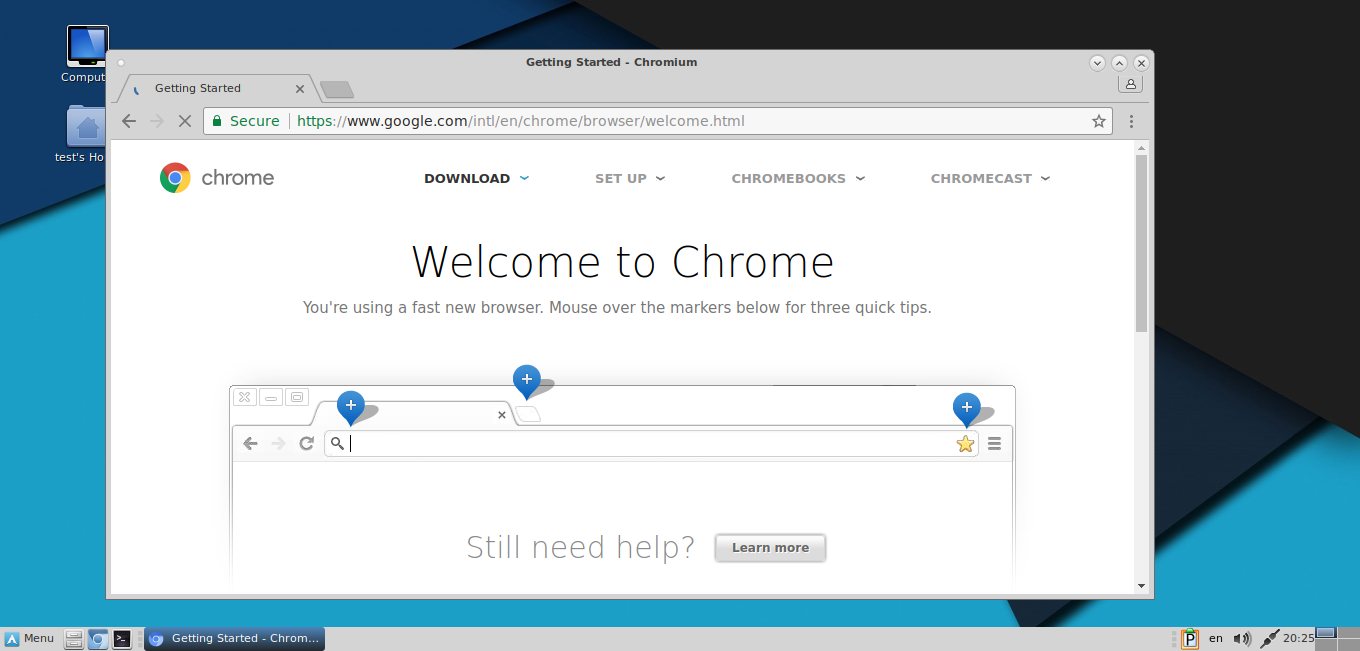
\includegraphics[width=300pt]{png/chromium}
		\caption{Web-browser Chromium}
	\end{figure}

	\newpage
	\subsection{Terminal Emulator}
	
	Terminal emulator merupakan program untuk mengakses \textit{interactive shell} dari sistem Unix-like (termasuk Linux).
	Shell yang digunakan oleh Arch Linux secara default adalah Bash.
	Sedangkan program terminal emulator yang digunakan AchmadiOS adalah bawaan MATE Desktop (mate-terminal). 
	
	Untuk memanggil mate-terminal, dapat dilakukan dengan cara:
	
	\begin{itemize}
		\item Shortcut Terminal di panel
		\item melalui klik \textbf{Menu}, kemudian \textbf{System Tools}, kemudian \textbf{MATE Terminal} 
		
		\begin{figure}[h]
			\centering
			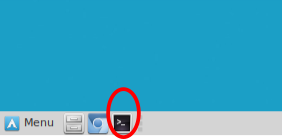
\includegraphics[width=200pt]{png/panelterminal}
			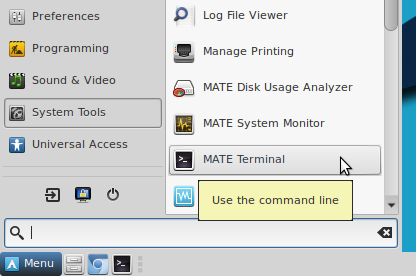
\includegraphics[width=200pt]{png/termmenu}
		\end{figure}
	
		\item dengan shortcut keyboard \keys{\ctrl + \Alt + t}
	\end{itemize}

	Maka jendela terminal emulator akan muncul dan anda dapat melakukan banyak hal terhadap komputer anda melalui terminal emulator.
	Perlu diketahui bahwa \textit{interactive shell} sifat prosesnya adalah \textit{forkable} yang artinya anda dapat membuka terminal sebanyak mungkin.
	Silahkan merujuk kepada tutorial lain tentang penggunaan terminal di sistem Linux.
	
	\begin{figure}[h]
		\centering
		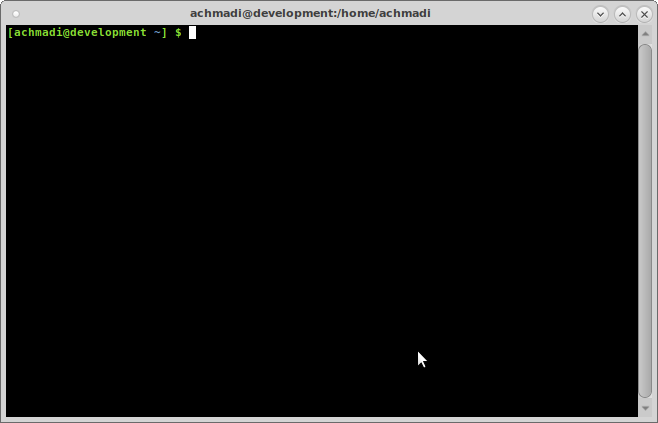
\includegraphics[width=250pt]{png/term_1}
		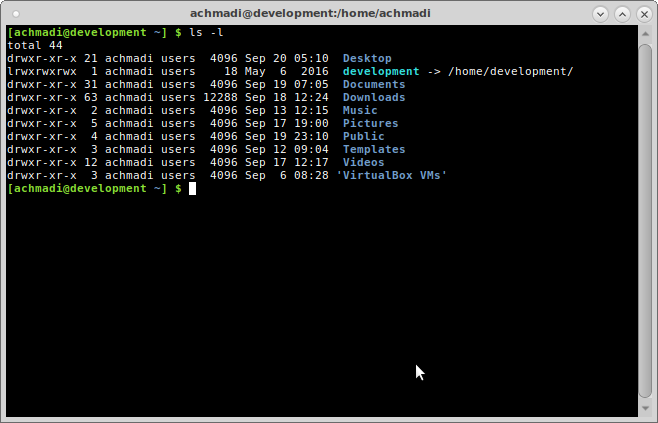
\includegraphics[width=250pt]{png/term_2}
		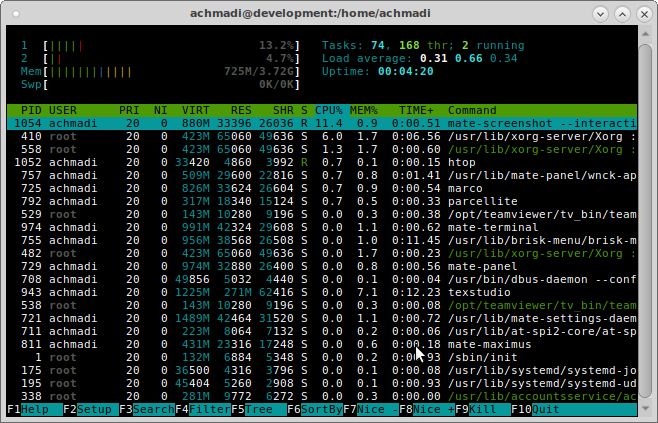
\includegraphics[width=250pt]{png/term_3}
		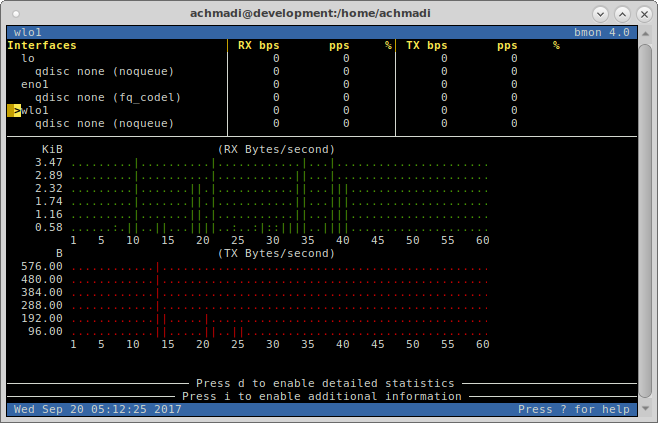
\includegraphics[width=250pt]{png/term_4}
		\caption{4 screenshot contoh pemakaian terminal}
	\end{figure}
	  
	\newpage
	\section{Pengaturan Dasar}

	Berikut adalah penjelasan beberapa pengaturan dasar.
	
	\subsection{Ganti Wallpaper}
	
	Anda dapat mengganti wallpaper desktop anda baik dengan wallpaper yang tersedia maupun anda gambar tambahan sendiri.
	Untuk ganti wallpaper, klik kanan desktop di bagian mana saja yang kosong
	Maka akan muncul context-menu sebagai berikut:
	
	\begin{figure}[h]
		\centering
		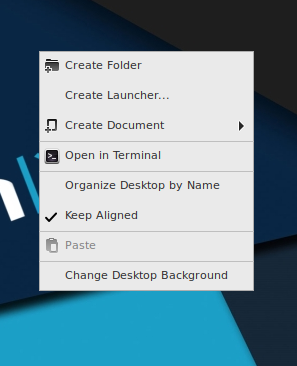
\includegraphics[width=200pt]{png/contextmenu}
		\caption{Context Menu pada desktop}
	\end{figure} 

	Anda klik menu \textbf{Change Desktop Background} (paling bawah)
	Maka akan muncul dialog berikut
	
	\begin{figure}[h]
		\centering
		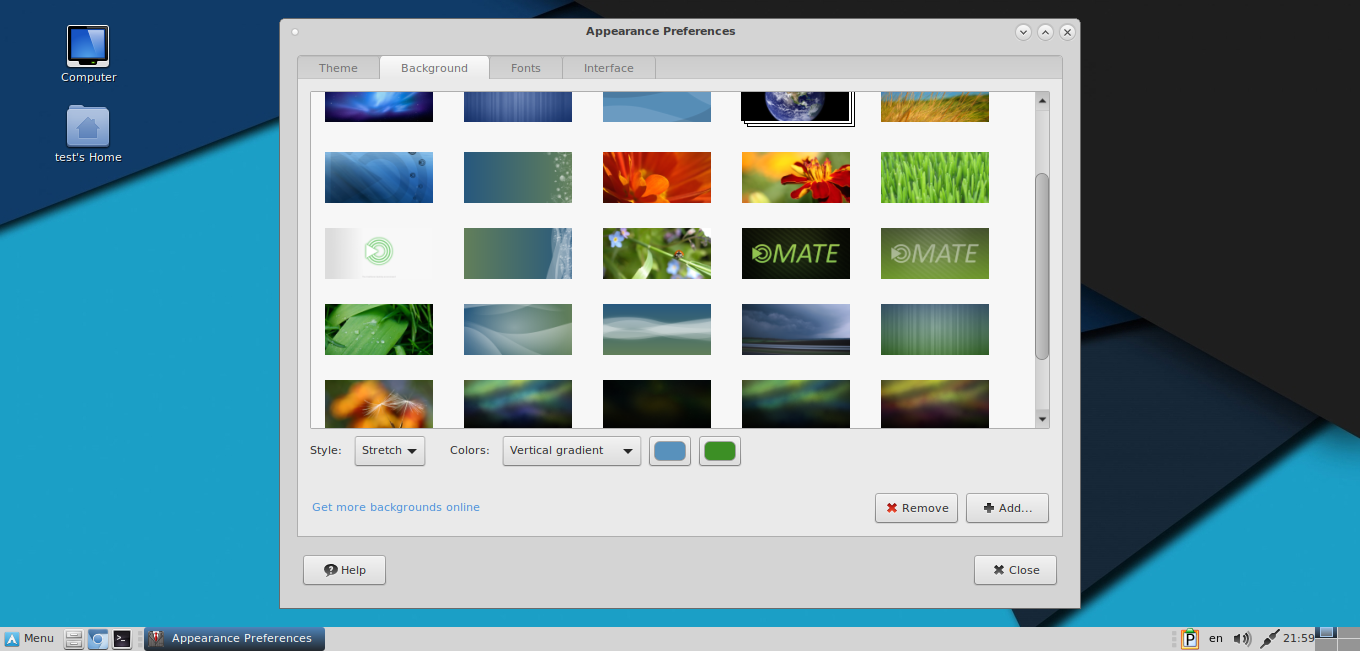
\includegraphics[width=300pt]{png/wallpaperdlg}
		\caption{Dialog Pengaturan Wallpaper}
	\end{figure}
	
	Anda tinggal klik gambar mana yang dipilih maka otomatis wallpaper desktop akan berubah.
	\newpage
	\begin{figure}[h]
		\centering
		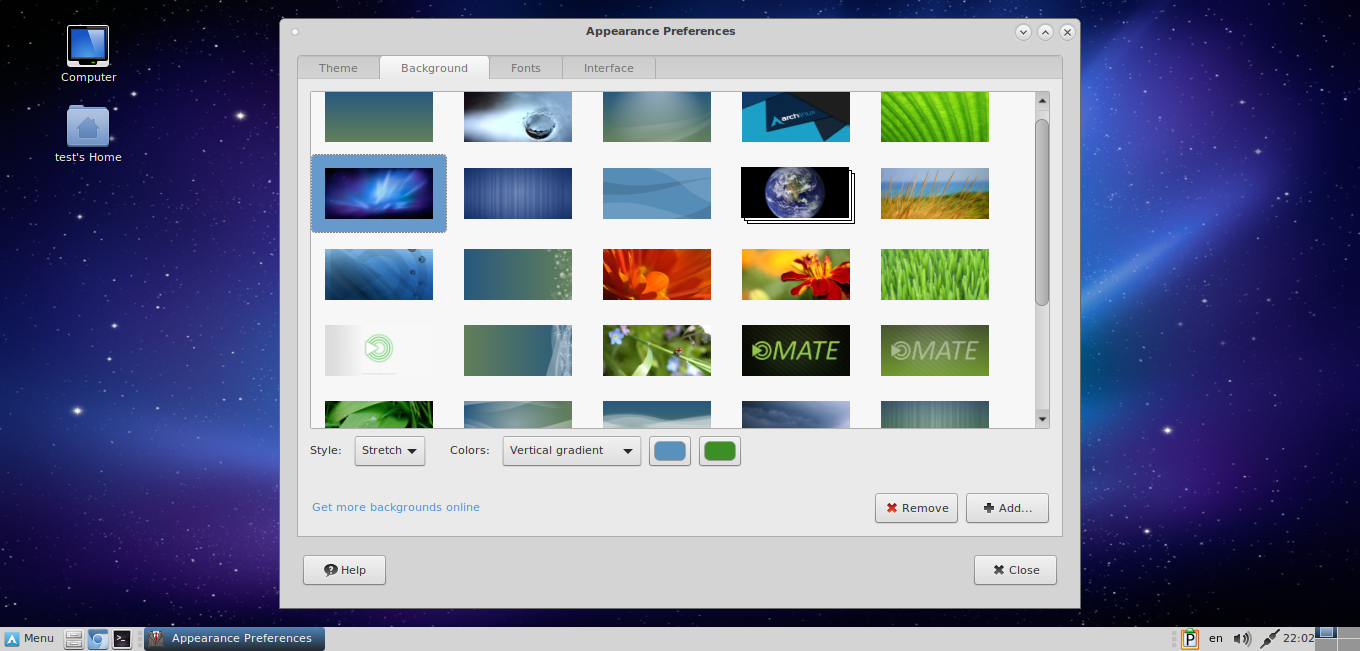
\includegraphics[width=300pt]{png/wallpaperdlg2}
		\caption{Pengaturan Wallpaper}
	\end{figure}

	Anda pun dapat menambah gambar dengan tombol \textbf{Add} yang ada di pojok kanan bawah dialog (dilingkari merah)
	
	\begin{figure}[h]
		\centering
		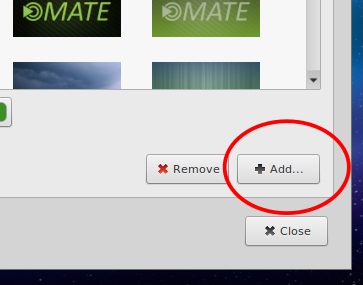
\includegraphics[width=200pt]{png/wallpaperadd}
		\caption{Tombol menambah Wallpaper}
	\end{figure}   

	Selanjutnya anda tinggal mencari gambar yang akan ditambahkan
	
	\begin{figure}[h]
		\centering
		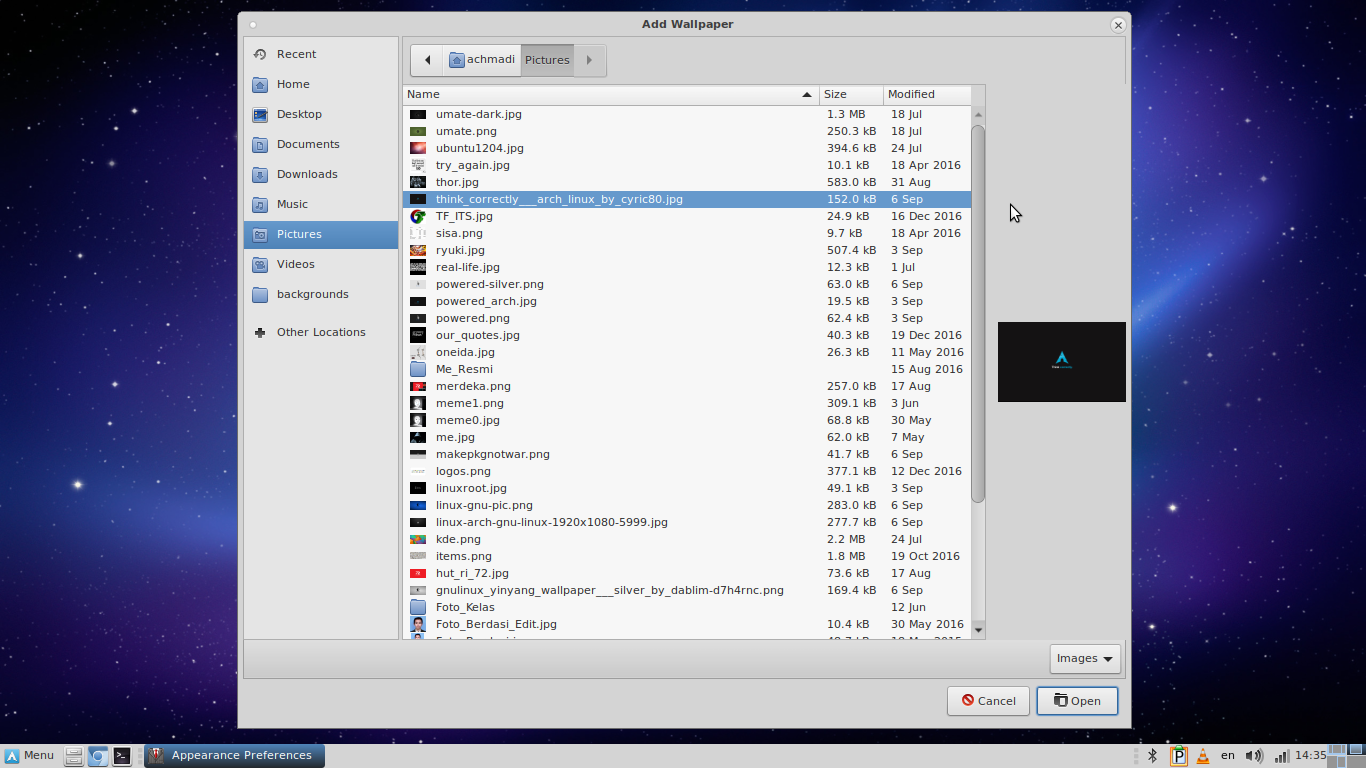
\includegraphics[width=300pt]{png/wallpaperadd2}
		\caption{Pilih Gambar Wallpaper}
	\end{figure}

	\newpage
	\subsection{Menyambung Koneksi Wifi}

	Untuk sambungan Ethernet, otomatis akan terhubung jika jaringan telah diatur dengan benar.
	Untuk sambungan wifi, klik icon koneksi pada system-tray (lingkaran merah)
	
	\begin{figure}[h]
		\centering
		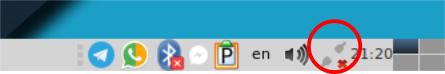
\includegraphics[width=200pt]{png/systraywifi}
		\caption{Icon Wifi pada systray}
	\end{figure}

	apabila icon tersebut diklik dan wifi sudah ON, maka akan tampil pilihan wifi yang tersedia
	
	\begin{figure}[h]
		\centering
		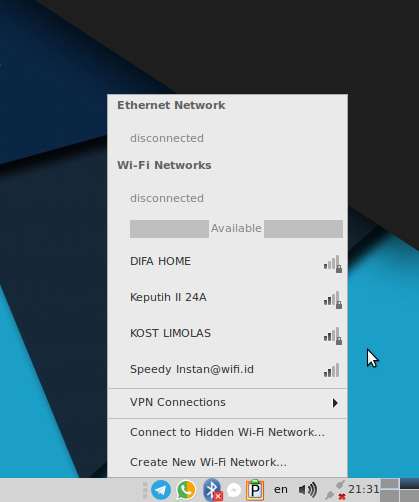
\includegraphics[width=200pt]{png/wifi}
		\caption{Pilihan wifi}
	\end{figure}
	
	Pilih Wifi yang anda bisa akses. 
	Apabila terdapat otentifikasi maka akan muncul dialog untuk anda memasukkan password.
	
	\begin{figure}[h]
		\centering
		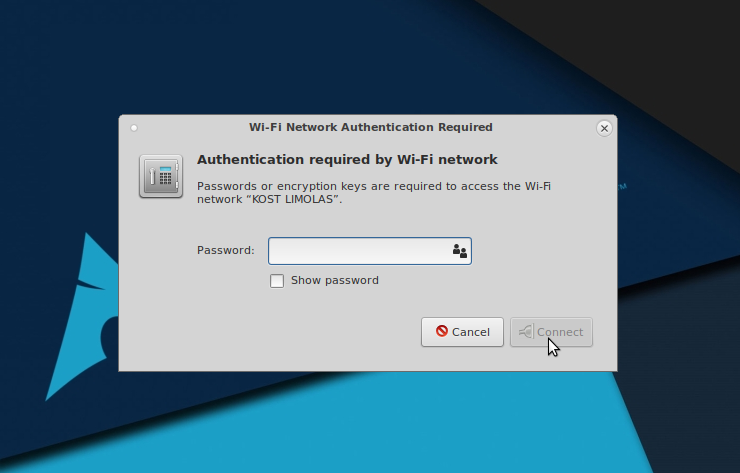
\includegraphics[width=200pt]{png/wifipass}
		\caption{Password wifi}
	\end{figure}

	\newpage
	
	\subsection{Sambungan Proxy}
	
	Apabila anda mengakses internet dibawah proxy server, anda dapat mengatur proxy server melalui menu.
	Klik \textbf{Menu}, kemudian \textbf{Preferences}, kemudian \textbf{Network Proxy}. 
	
	\begin{figure}[h]
		\centering
		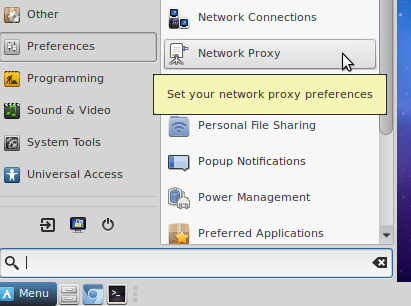
\includegraphics[width=250pt]{png/menuproxy}
		\caption{memanggil Proxy setting dari Menu}
	\end{figure}

	Jika dijalankan maka akan muncul dialog seperti dibawah ini.
	Anda dapat memasukkan URL atau IP proxy server anda seperti dicontohkan disini.
	
	\begin{figure}[h]
		\centering
		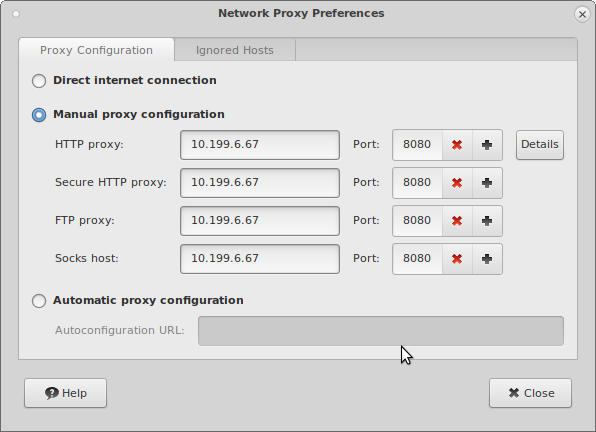
\includegraphics[width=250pt]{png/proxydlg}
		\caption{Dialog Proxy setting}
	\end{figure}
	
	\newpage
	
	\subsection{Audio Setting}
	
	Anda dapat mengatur volume audio anda melalui icon Audio yang ada di systray (dilingkari merah)
	
	\begin{figure}[h]
		\centering
		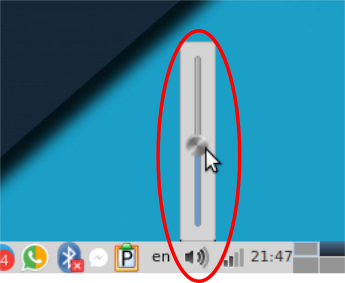
\includegraphics[width=200pt]{png/systrayaudio}
		\caption{Icon Audio pada systray}
	\end{figure}

	Untuk pengaturan lebih jauh, anda bisa Klik Kanan icon tersebut dan klik menu \textbf{Sound Preference}
	Maka akan muncul dialog pengaturan yang lebih lengkap.
	
	\begin{figure}[h]
		\centering
		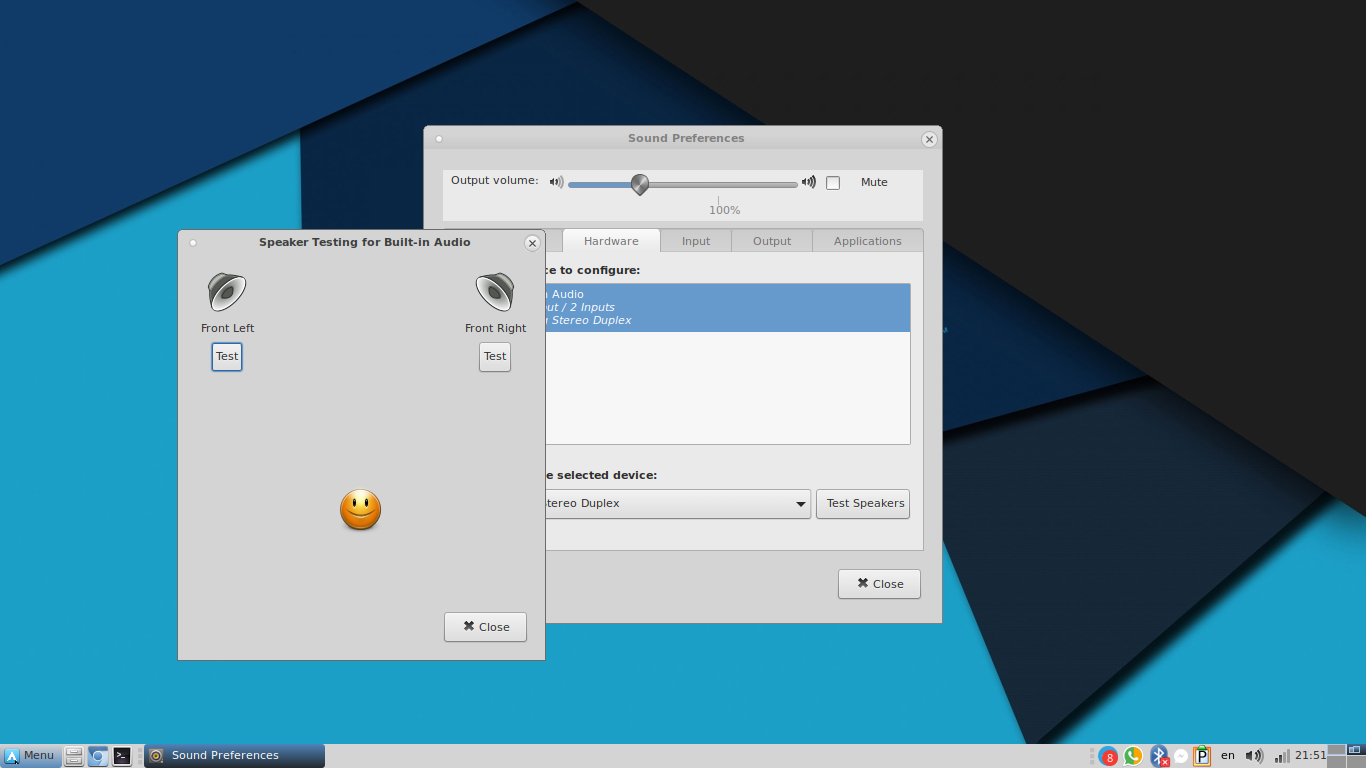
\includegraphics[width=300pt]{png/audiodlg}
		\caption{Dialog Pengaturan Audio}
	\end{figure}
	
	\newpage
	\section{Instalasi AchmadiOS ke USB}
	
	\subsection{ISO File}
	Berikut adalah tutorial menulis Arch Linux ISO ke USB
	
	Sebelum instalasi, file ISO dapat didownload di \href{https://drive.google.com/open?id=0B1r9uekKJ7Z0ellkTVdmdUdYQmM}{disini}
	 
	Dalam directory tersebut, tersedia dua file:
	\begin{itemize}
		\item achmadiOS-x86\_64.iso. Merupakan ISO Arch Linux Custom berarsitektur 64bit (x86\_64)
		\item download.txt. Berisi url download dan MD5sum
	\end{itemize}

	kemudian selain file ISO di atas, juga diperlukan USB flashdisk minimal 4GB.
	
	\textbf{(Catatan: Backup dahulu isi flashdisk karena pastinya akan diformat)}

	\subsection{Ubuntu/LinuxMint}
	
	untuk menulis AchmadiOS ke USB di distro Ubuntu/LinuxMint, dibutuhkan program tambahan syslinux dan parted.
	Perintah instalasi di Ubuntu/LinuxMint (pastikan terhubung internet):
	 
	\begin{minted}[frame=lines,fontsize=\footnotesize]{bash}
sudo apt-get install syslinux syslinux-common mtools dosfstools parted
	\end{minted}
	
	Berikut langkah-langkahnya:
	
	\begin{enumerate}
		\item cek file ISO dan mount ke /tmp/arch-iso.
		\begin{minted}[frame=lines,fontsize=\footnotesize]{bash}
ls -l 
mv achmadiOS-x86_64.iso archlinux-achmadi-x86_64.iso
sudo mkdir /tmp/arch-iso 
sudo mount archlinux-achmadi-x86_64.iso /tmp/arch-iso
		\end{minted} 
		
		\begin{figure}[h]
			\centering
			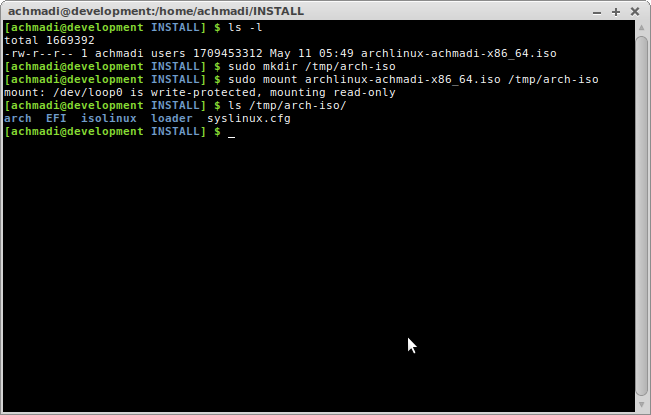
\includegraphics[width=250pt]{usbubuntu/step_1}
		\end{figure} 
	
		\item cek alamat USB Flashdisk.
		Biasanya alamat USB FD adalah /dev/sdb, /dev/sdc, dst, sementara alamat /dev/sda ditempati oleh Hardisk lokal, namun ini tidak selalu.
		(\textbf{PERINGATAN}: Jangan sampai tertukar, karena akan ada proses memformat sehingga seluruh data bisa \textbf{TERHAPUS} )
		
		\begin{minted}[frame=lines,fontsize=\footnotesize]{bash}
sudo fdisk -l
		\end{minted} 
		
		\newpage
		\begin{figure}[h]
			\centering
			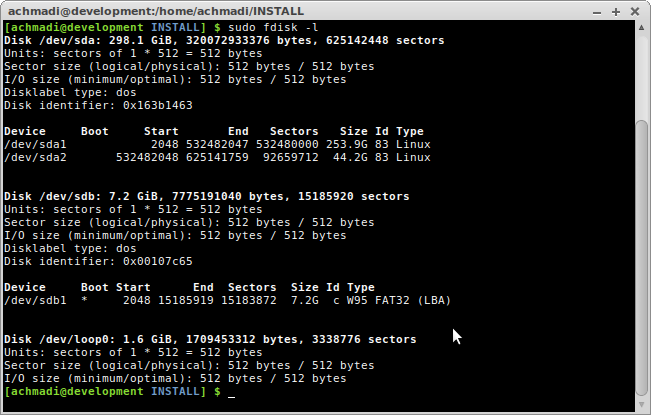
\includegraphics[width=250pt]{usbubuntu/step_2}
		\end{figure}
	
		\item Terlihat alamat USB FD adalah \textbf{/dev/sdb1}.
		Kemudian unmount USB FD dan tulis ulang Tabel Partisi nya (seluruh data akan \textbf{TERHAPUS}).
		Selanjutnya masuk program cfdisk untuk mempartisi ulang USB FD
		
		\begin{minted}[frame=lines,fontsize=\footnotesize]{bash}
sudo umount /dev/sdb1 
sudo dd bs=1k count=2048 if=/dev/zero of=/dev/sdb 
sudo cfdisk /dev/sdb
		\end{minted} 	
		
		\begin{figure}[h]
			\centering
			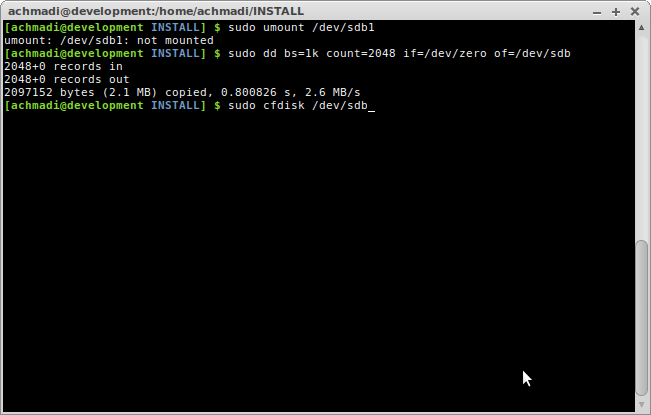
\includegraphics[width=250pt]{usbubuntu/step_3}
		\end{figure}
	
		\item Selanjutnya akan tampil pilihan jenis partisi baru untuk USB FD.
		Pilih dengan tombol panah \textbf{dos} dan tekan Enter (\keys{\return}).
		
		\begin{figure}[h]
			\centering
			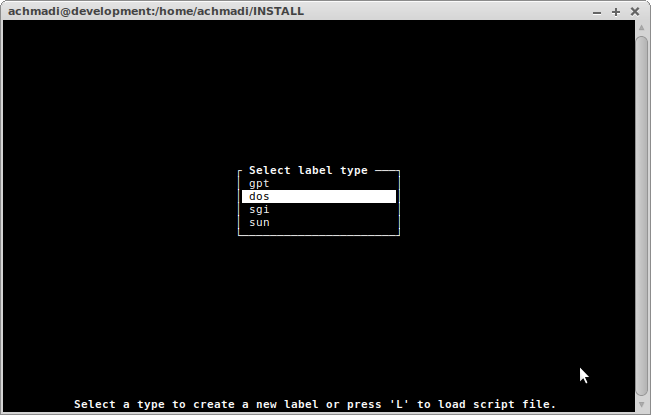
\includegraphics[width=250pt]{usbubuntu/step_4}
		\end{figure}	
	
		\item Selanjutnya tampil ruang kosong USB FD dan pilihan untuk membuat partisi baru.
		Pilih dengan tombol panah \textbf{New} dan tekan Enter (\keys{\return}).
		
		\newpage
		
		\begin{figure}[h]
			\centering
			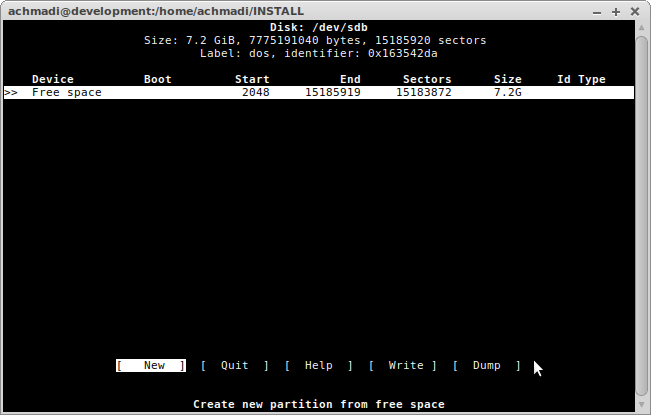
\includegraphics[width=250pt]{usbubuntu/step_5}
		\end{figure}
	
		\item Ambil semua ukuran ruang kosong (biarkan saja nilai yang ada) dan tekan Enter(\keys{\return}).
		
		\begin{figure}[h]
			\centering
			\includegraphics[width=250pt]{usbubuntu/step_6}
		\end{figure}
	
		\item Pilih jenis partisi dengan tombol panah \textbf{Primary} dan tekan Enter.
		
		\begin{figure}[h]
			\centering
			\includegraphics[width=250pt]{usbubuntu/step_7}
		\end{figure}
	
		\item Kemudian tersedia pilihan untuk mengatur partisi.
		Pilih dengan tombol panah \textbf{Write} dan tekan Enter.
		
		\newpage
		\begin{figure}[h]
			\centering
			\includegraphics[width=250pt]{usbubuntu/step_8}
		\end{figure}
	
		\item Kemudian muncul konfirmasi. Ketik \textbf{yes} dan tekan Enter.
		
		\begin{figure}[h]
			\centering
			\includegraphics[width=250pt]{usbubuntu/step_9}
		\end{figure}
	
		\item Selesai proses partisi ulang USB FD, maka bisa keluar dari program cfdisk. 
		Pilih dengan tombol panah \textbf{Quit} dan tekan Enter.
		
		\begin{figure}[h]
			\centering
			\includegraphics[width=250pt]{usbubuntu/step_10}
			\includegraphics[width=250pt]{usbubuntu/step_11}
		\end{figure}
	
		\item selanjutnya USB FD di format sebagai FAT32 dan di beri Volume Label yang sama dengan label ISO image, kemudian ditulis MBR (Master Boot Record)
		\begin{minted}[frame=lines,fontsize=\footnotesize]{bash}
export ISO_LABEL=$(cat /tmp/arch-iso/arch/boot/syslinux/archiso_sys64.cfg \
 | grep archisolabel \
 | cut -d\= -f3) 
sudo mkfs.vfat /dev/sdb1 
sudo dosfslabel /dev/sdb1 "$ISO_LABEL" 
sudo dd conv=notrunc bs=440 count=1 if=/usr/lib/syslinux/bios/mbr.bin of=/dev/sdb
		\end{minted} 		
		
		\newpage
		\begin{figure}[h]
			\centering
			\includegraphics[width=250pt]{usbubuntu/step_12}
		\end{figure}
	
		\item Selanjutnya mount USB FD ke /tmp/arch-usb dengan UID sendiri dan akses RW.
		
		\begin{figure}[h]
			\centering
			\includegraphics[width=250pt]{usbubuntu/step_13}
		\end{figure}
	
		\item Selanjutnya copy semua file dari ISO image (mounted di /tmp/arch-iso) ke USB FD (mounted di /tmp/arch-usb).
		
		\begin{figure}[h]
			\centering
			\includegraphics[width=250pt]{usbubuntu/step_14}
			\includegraphics[width=250pt]{usbubuntu/step_15}
		\end{figure} 
	
		\item Aktifkan Boot Flag di FD USB dan install Syslinux loader.
		
		\begin{minted}[frame=lines,fontsize=\footnotesize]{bash}
sudo parted /dev/sdb set 1 boot on 
sudo syslinux /dev/sdb1
		\end{minted} 	
		\newpage
		\begin{figure}[h]
			\centering
			\includegraphics[width=250pt]{usbubuntu/step_16}
		\end{figure}
	
		\item Terakhir, unmount USB FD dan ISO image. 

		\begin{minted}[frame=lines,fontsize=\footnotesize]{bash}
sudo umount /tmp/arch-iso 
sudo umount /tmp/arch-usb
		\end{minted} 
		
		\begin{figure}[h]
			\centering
			\includegraphics[width=250pt]{usbubuntu/step_17}
		\end{figure}		
		
		\item Selesai, USB FD siap dicoba.
		
	\end{enumerate}

	\newpage
	\subsection{Arch Linux}
	
	Untuk pengguna Arch Linux, dapat menggunakan tools yang telah saya tulis.
	PKGBUILD dapat didownload \href{https://github.com/mekatronik-achmadi/achmadi-usb/blob/master/PKGBUILD}{disini}.
	Sedangkan untuk pengguna AchmadiOS, sudah tersedia pre-installed
	
	Apabila sudah terinstal, anda dapat memanggil tool ini dengan cara:
	\begin{itemize}
		\item melalui perintah di terminal
		\begin{minted}[frame=lines,fontsize=\footnotesize]{bash}
sudo /usr/share/achmadi-usb/arch-usb_gui.py
		\end{minted}
		
		\item melalui klik \textbf{Menu}, kemudian \textbf{System Tools}, kemudian \textbf{USB Arch Linux} 
		
		\begin{figure}[h]
			\centering
			\includegraphics[width=250pt]{usbarch/menu}
		\end{figure}
	\end{itemize}

	maka akan muncul dialog seperti ini
	
	\begin{figure}[h]
		\centering
		\includegraphics[width=250pt]{usbarch/dialog}
	\end{figure}

	selanjutnya berikut adalah langkah-langkah membuat USB Arch Linux:
	\begin{itemize}
		\item cek alamat USB Flashdisk.
		Biasanya alamat USB FD adalah /dev/sdb, /dev/sdc, dst, sementara alamat /dev/sda ditempati oleh Hardisk lokal, namun ini tidak selalu.
		(\textbf{PERINGATAN}: Jangan sampai tertukar, karena akan ada proses memformat sehingga seluruh data bisa \textbf{TERHAPUS} )
		
		\begin{minted}[frame=lines,fontsize=\footnotesize]{bash}
sudo fdisk -l
		\end{minted} 
		
		\newpage
		\begin{figure}[h]
			\centering
			\includegraphics[width=250pt]{usbarch/usb}
		\end{figure}
	
		\item selanjutnya panggil program \textbf{USB Arch Linux}.
		Klik tombol \textbf{Open} untuk mencari file ISO Arch Linux yang akan ditulis.
		
		\begin{figure}[h]
			\centering
			\includegraphics[width=250pt]{usbarch/step_1}
		\end{figure}
	
		\item apabila partisi USB di alamat \textbf{/dev/sdb1} maka alamat device USB adalah \textbf{/dev/sdb}.
		Jangan ditukar antara alamat partisi dan device.
		
		\begin{figure}[h]
			\centering
			\includegraphics[width=250pt]{usbarch/step_2}
		\end{figure}
	
		\item tekan tombol \textbf{Create} untuk memulai proses. 
		Akan keluar dialog konfirmasi.
		Cek kembali alamat yang telah di entri.
		Tekan \textbf{OK} untuk melanjutkan.	
		
		\newpage
		\begin{figure}[h]
			\centering
			\includegraphics[width=250pt]{usbarch/step_3}
		\end{figure}
	
		\item proses berjalan dan tunggu hingga selesai
		
		 \begin{figure}[h]
		 	\centering
		 	\includegraphics[width=250pt]{usbarch/step_4}
		 	\includegraphics[width=250pt]{usbarch/step_5}
		 \end{figure}
	 
	 	\item setelah proses selesai, tutup semua jendela dan USB AchmadiOS siap dicoba.
	 	
	 	\begin{figure}[h]
	 		\centering
	 		\includegraphics[width=250pt]{usbarch/step_6}
	 	\end{figure}
		 
	\end{itemize}

	\newpage
	\subsection{Windows}
	
	untuk menulis AchmadiOS ke USB di distro Windows, dibutuhkan program tambahan Rufus.
	Anda dapat mendownloadnya di situs resmi Rufus \href{https://rufus.akeo.ie/}{disini}.
	Untuk dapat berjalan sebagaimana seharusnya dibutuhkan library syslinux.
	Rufus secara otomatis akan mendownload library syslinux.
	Anda dapat mendownload Rufus plus syslinux \href{http://www.mediafire.com/download/5gdb8z98zg8sgxj/rufus.zip}{disini} 
	
	Berikut adalah langkah-langkahnya:
	\begin{enumerate}
		\item Pastikan sudah mendownload ISO dan Rufus secara lengkap.
		\begin{figure}[h]
			\centering
			\includegraphics[width=250pt]{usbwin/step_1}
			\includegraphics[width=250pt]{usbwin/step_2}
		\end{figure}
	
		\item Jalankan Rufus-2.5.exe dan akan keluar tampilan berikut.
		\begin{figure}[h]
			\centering
			\includegraphics[width=250pt]{usbwin/step_3}
		\end{figure}
	
		\item Kemudian \textbf{(1)} Ganti Volume Label ke ARCH\_LINUX karena sistem live dari Arch Linux secara default mencari root filesystem berdasarkan label,
		selanjutnya \textbf{(2)} pilih sumber bootable ISO Image
		dan \textbf{(3)} cari file ISO image tersebut.
		
		\begin{figure}[h]
			\centering
			\includegraphics[width=250pt]{usbwin/step_4}
			\includegraphics[width=250pt]{usbwin/step_5}
		\end{figure}
	
		\item Pastikan kembali hasilnya seperti ini.
		
		\newpage
		\begin{figure}[h]
			\centering
			\includegraphics[width=250pt]{usbwin/step_6}
		\end{figure}
	
		\item Klik Start, maka akan muncul konfirmasi yang bertanya apakah yakin akan memformat USB FlashDisk (seluruh data akan \textbf{TERHAPUS}),
		jika sudah yakin pilih OK.

		\begin{figure}[h]
			\centering
			\includegraphics[width=250pt]{usbwin/step_7}
		\end{figure}
	
		\item Proses berjalan dan tinggal menunggu selesai dan USB FlashDisk siap dicoba.
		
		\begin{figure}[h]
			\centering
			\includegraphics[width=250pt]{usbwin/step_8}
			\includegraphics[width=250pt]{usbwin/step_9}
		\end{figure}
		
		\begin{center}
			\includegraphics[width=250pt]{usbwin/step_10}
		\end{center}
			
	\end{enumerate}

	\newpage
	\section{Instalasi AchmadiOS ke HDD}
	
	Berikut adalah tutorial instalasi AchmadiOS ke harddisk drive (HDD) untuk komputer/laptop yang memiliki CPU x86\_64 (64-bit).
	Disarankan untuk konsultasi kepada yang telah paham atau pernah instalasi suatu distro GNU/Linux.
	Proses instalasi suatu OS, baik Windows, Mac, BSD, atau GNU/Linux, \textbf{sangat beresiko kehilangan data} jika tidak hati-hati.
	
	\subsection{Persiapan}
	Persiapan yang pertama adalah menyiapkan media booting AchmadiOS.
	Baik dengan menulis ISO AchmadiOS ke DVD atau USB Flashdisk.
	Penulis lebih menyarankan USB Flashdisk sebagai media booting.
	Silahkan mengikuti bab sebelumnya untuk bagaimana menulis ISO ke USB Flashdisk.
	
	Persiapan selanjutnya adalah menyiapkan ruang kosong pada HDD.
	Silahkan backup data terlebih dahulu apabila akan mengolah suatu partisi HDD.
	Ukuran minimal ruang yang dibutuhkan adalah:
	\begin{itemize}
		\item partisi root (wajib). Ukuran minimal 10GB
		\item partisi home (opsional). Ukuran sesuai kebutuhan
		\item partisi swap (opsional). Ukuran minimal sama dengan ukuran RAM
	\end{itemize}
	Penulis tidak merekomendasikan penggunaan partisi SWAP apabila ukuran RAM 4GB atau lebih.
	
	Persiapan terakhir adalah menyiapkan komputer/laptop untuk booting pertamanya adalah USB atau DVD (tergantung media booting yang anda pilih).
	Silahkan merujuk kepada dokumentasi sistem BIOS/UEFI dari vendor komputer/laptop anda. 
	
	\newpage
	\subsection{Boot USB/DVD}
	selanjutnya adalah booting USB/DVD ke komputer/laptop yang akan diinstall.
	Untuk booting DVD atau USB-legacy (BIOS), maka tampilan seperti sebelah kiri.
	Sedangkan untuk USB UEFI maka tampilan seperti sebelah kanan.
	Tekan Enter (\keys{\return}) untuk melanjutkan.
	
	\begin{figure}[h]
		\centering
		\includegraphics[width=250pt]{installhdd/step_1a}
		\includegraphics[width=250pt]{installhdd/step_1b}
	\end{figure}  

	Tunggu beberapa saat untuk proses booting.
	Setelah itu akan masuk tampilan login.
	Default username adalah live tanpa password.
	Klik tombol \textbf{Log In} atau Enter (\keys{\return}) untuk melanjutkan.
	Maka anda akan masuk tampilan desktop.
	
	\begin{figure}[h]
		\centering
		\includegraphics[width=250pt]{installhdd/step_2}
		\includegraphics[width=250pt]{installhdd/step_3}
	\end{figure} 
	
	\newpage
	\subsection{Program Installer}
	Selanjutnya panggil program installer.
	Anda dapat memanggilnya dari menu.
	Klik \textbf{Menu}, kemudian \textbf{Administration}, dan kemudian \textbf{Live Installer}. 
	
	\begin{figure}[h]
		\centering
		\includegraphics[width=200pt]{installhdd/step_4}
		\caption{Menu Live Installer}
	\end{figure}

	Maka akan muncul dialog installer sederhana.
	Dengan program inilah AchmadiOS akan diinstal.
	
	\begin{figure}[h]
		\centering
		\includegraphics[width=200pt]{installhdd/step_5}
		\caption{Dialog Live Installer}
	\end{figure}   
	
	\newpage
	\subsection{Partisi dan Format HDD}
	
	Selanjutnya adalah mempartisi HDD.
	Proses partisi HDD disini hanyalah sebagai contoh.
	Contoh disini hanyalah proses membagi dan memformat partisi HDD dari kondisi awal kosong (tanpa ada partisi apapun).
	Proses partisi HDD pada komputer/laptop anda bisa jadi akan berbeda.
	
	Untuk memanggil pengolah partisi, tekan tombol Partition Editor pada dialog Live Installer (lingkaran merah).
	
	\begin{figure}[h]
		\centering
		\includegraphics[width=200pt]{installhdd/step_6}
		\caption{Panggil partition Editor}
	\end{figure}

	Maka akan muncul jendela \textbf{GParted}, program partisi editor bawaan AchmadiOS.
	
	\begin{figure}[h]
		\centering
		\includegraphics[width=250pt]{installhdd/step_7}
		\caption{Jendela GParted}
	\end{figure}

	Selanjutnya buat partisi baru. Tekan menu \textbf{Partition} dan kemudian \textbf{New}.
	
	Maka akan muncul dialog pengaturan partisi baru.
	Entry \textbf{New size (MiB)} diisi 10000.
	Entry \textbf{File system}  diisi ext4.
	Partisi ini akan digunakan sebagai partisi root sehingga butuh minimal 10GB.
	
	\newpage
	\begin{figure}[h]
		\centering
		\includegraphics[width=250pt]{installhdd/step_8}
		\includegraphics[width=250pt]{installhdd/step_9}
	\end{figure}

	Ulangi proses serupa dengan seluruh ukuran ruang tersisa.
	Entry \textbf{New size (MiB)} biarkan apa adanya.
	Entry \textbf{File system}  diisi ext4.
	Partisi ini akan digunakan sebagai partisi home yang sifatnya sebenarnya opsional.
	Sehingga pembagian partisi menjadi seperti pada gambar kanan.
	
	\begin{figure}[h]
		\centering
		\includegraphics[width=250pt]{installhdd/step_10}
		\includegraphics[width=250pt]{installhdd/step_11}
	\end{figure}

	Selanjutnya tekan \textbf{Edit} dan \textbf{Apply All Operations}.
	Akan muncul jendela konfirmasi. 
	Pilih \textbf{Apply} untuk melanjutkan.
	Apabila ada data dalam partisi ini, maka data akan \textbf{terhapus}.
	
	\newpage
	\begin{figure}[h]
		\centering
		\includegraphics[width=250pt]{installhdd/step_12}
		\includegraphics[width=250pt]{installhdd/step_13}
	\end{figure}

	Tunggu beberapa saat dan proses pemformatan akan selesai.
	Anda dapat menutup jendela GParted setelah proses pengolahan partisi selesai.
	
	\begin{figure}[h]
		\centering
		\includegraphics[width=250pt]{installhdd/step_14}
		\includegraphics[width=250pt]{installhdd/step_15}
	\end{figure}
	
	Sampai pada proses ini, maka yang perlu diingat adalah:
	\begin{itemize}
		\item alamat partisi root adalah \textbf{/dev/sda1}. Partisi root ini wajib ada
		\item alamat partisi home adalah \textbf{/dev/sda2}. Partisi home ini opsional
		\item alamat device hdd adalah \textbf{/dev/sda} (sesuai alamat partisi root namun tanpa akhiran angka)
	\end{itemize}

	Apabila anda lupa, anda dapat kembali klik "Partition Editor" pada dialog Live Installer untuk sekedar melihat partisi HDD.
	
	\newpage
	\subsection{Install AchmadiOS ke HDD}
	
	Selanjutnya anda akan kembali kepada dialog Live Installer.
	Berikut adalah penjelasan entry yang bisa anda inputkan ke dalam dialog:
	
	\begin{itemize}
		\item \textbf{User Name}. Nama pengguna default. Anda dapat isi sesuai selera. disini dicontohkan \textbf{adi}
		\item \textbf{Host Name}. Nama komputer anda. Anda dapat isi sesuai selera. disini dicontohkan \textbf{archlinux}
		\item \textbf{Method}. Metode deployment yang digunakan saat instalasi. Terdapat dua pilihan.
		\begin{itemize}
			\item \textbf{rsync}. Opsi ini lebih lambat namun mampu dijalankan oleh komputer/laptop dengan RAM dibawah 4GB.
			\item \textbf{unsquashfs}. Opsi ini lebih cepat namun hanya untuk komputer/laptop dengan RAM 4GB atau lebih.
		\end{itemize}
		disini dicontohkan menggunakan rsync karena RAM yang tersedia hanya 1GB.
		\item \textbf{Root (/)}. Alamat partisi root. Disini dicontohkan /dev/sda1 sebagai sub-bab sebelumnya
		\item \textbf{Home (/home/)}. Alamat partisi home. Centang checkbox untuk mengisinya.
		Disini dicontohkan /dev/sda2 sebagai sub-bab sebelumnya.
		\item \textbf{Swap}.Alamat partisi swap. Centang checkbox untuk mengisinya.
		Disini dicontohkan tidak menggunakan swap-area sehingga dibiarkan kosong dan checkbox tidak dicentang.
		\item \textbf{GRUB}. Alamat device HDD yang akan diinstal GRUB loader.
		Alamat GRUB mengacu kepada alamat partisi root namun tanpa akhiran angka. 
		Disini dicontohkan /dev/sda sebagai sub-bab sebelumnya.
	\end{itemize}

	\begin{figure}[h]
		\centering
		\includegraphics[width=200pt]{installhdd/step_16}
		\caption{Entry instalasi}
	\end{figure}

	Selanjutnya klik \textbf{INSTALL} (dilingkari merah).
	Maka akan muncul dialog konfirmasi.
	Klik \textbf{OK} untuk melanjutkan.
	
	\newpage
	\begin{figure}[h]
		\centering
		\includegraphics[width=250pt]{installhdd/step_17}
		\includegraphics[width=250pt]{installhdd/step_18}
	\end{figure}

	Maka proses instalasi akan dimulai dan tunggu hingga selesai.
	
	\begin{figure}[h]
		\centering
		\includegraphics[width=250pt]{installhdd/step_19}
		\includegraphics[width=250pt]{installhdd/step_20}
	\end{figure}

	Setelah selesai maka akan muncul jendela pemberitahuan.
	Klik \textbf{OK} untuk menutup jendela pemberitahuan tersebut.
	Selanjutnya anda dapat menutup jendela dialog Live Installer dan GParted (bila masih ada).
	Kemudian matikan/restart komputer/laptop anda dan boot ke HDD anda.
	
	\begin{figure}[h]
		\centering
		\includegraphics[width=250pt]{installhdd/step_21}
		\includegraphics[width=250pt]{installhdd/step_22}
	\end{figure}
	
	\newpage	
	\subsection{Pasca Instalasi}
	
	Setelah anda menginstal AchmadiOS ke HDD, anda dapat melakukan beberapa hal untuk menyesuaikan instalasi AchmadiOS anda.
	Berikut beberapa hal yang dapat anda lakukan setelah instalasi AchmadiOS.
	\begin{itemize}
		\item Autologin. Yaitu membuat secara default login ke akun anda tanpa melewati Login Manager setiap booting.
		Berikut perintah di terminal (ganti USERNAME dengan nama user anda).
		\begin{minted}[frame=lines,fontsize=\footnotesize]{bash}
sudo achmadi_autologin USERNAME
		\end{minted}
		
		\item Timezone. Yaitu menyesuaikan zona waktu.
		Untuk dapat melihat zona waktu yang tersedia, gunakan perintah di terminal:
		\begin{minted}[frame=lines,fontsize=\footnotesize]{bash}
achmadi_localtime list
		\end{minted}
		Tekan tombol \keys{q} untuk keluar.
		Disini dicontohkan zona waktu yang dipakai adalah zona waktu Jakarta.
		Maka perintahnya.
		\begin{minted}[frame=lines,fontsize=\footnotesize]{bash}
sudo achmadi_localtime Asia/Jakarta
		\end{minted}
		
		\item Password. Secara default user anda tidak memiliki password.
		Untuk memasang password, berikut perintah di terminal (ganti USERNAME dengan nama user anda):
		\begin{minted}[frame=lines,fontsize=\footnotesize]{bash}
sudo passwd USERNAME
		\end{minted}		 
		Anda akan diminta memasukkkan suatu password.
		Memang tidak tampil apapun saat anda mengetik karakter password anda.
		Namun sebenarnya karakter tersebut masuk.
		Tekan Enter (\keys{\return}) untuk melanjutkan.
		Anda akan diminta memasukkan password sekali lagi (sebagai konfirmasi).
		Tekan Enter (\keys{\return}) lagi jika telah selesai.
		Selanjutnya silahkan anda logout dan kembali login dengan password yang telah anda buat.
	\end{itemize}

	\newpage
	\section{Manajemen Paket (Repositori)}
	
	Bab ini adalah penjelasan manajemen paket software AchmadiOS.
	Karena pada dasarnya AchmadiOS adalah Arch Linux, maka manajemen paket yang digunakan identik dengan Arch Linux.
	Anda dapat mempelajari sistem manajemen paket Arch Linux karena tutorial ini hanya memberikan dasarnya saja.
	
	\subsection{Perkenalan}
	Pada dasarnya, sistem instalasi paket di semua OS tidaklah jauh berbeda. 
	Beberapa metode umum instalasi software yang ada saat ini antara lain:
	\begin{itemize}
		\item Instalasi dari sources. 
		Metode ini mem-building software dari sourcecode melalui proses kompilasi.
		Yang perlu disiapkan adalah toolchain kompilasi dan sourcecode.
		Metode ini sangat umum diterapkan di sistem diluar Linux.
		
		\item Instalasi dari binary siap pakai (pre-compiled) yang di distribusikan melalui paket software Installer.
		 Metode ini cukup mudah dan sudah umum diterapkan baik oleh Linux, Mac, BSD, dan terutama Windows.
		 
		\item Instalasi dari binary siap pakai (pre-compiled) yang di kumpulkan dalam satu lumbung server Repositori.
		Metode ini telah diterapkan di hampir semua sistem Linux dan BSD. 
		Kemudian diadopsi Android dengan Google-Play nya dan Apple dengan Apple-Store nya.
		
		\item Instalasi campuran yang mengkombinasikan 3 sistem instalasi sebelumnya.
		Arch Linux dikenal sangat fleksibel dalam instalasi karena mampu mengkombinasikan sistem instalasi yang berbeda.
	\end{itemize}

	Bab tutorial ini hanya mengacu kepada instalasi dari binary siap pakai (pre-compiled) yang di kumpulkan dalam satu lumbung server Repositori.
	Adapun metode instalasi kombinasi akan dijelaskan singkat pada bab selanjutnya.
	Perlu diketahui sebelumnya bab ini dan bab setelahnya akan berpusat pada penggunaan terminal dibandingkan GUI.
	
	\subsection{Penamaan File Paket}
	File paket Arch Linux memiliki standar penamaan yang dipisah tanda strip (-).
	Yaitu:
	\begin{minted}[frame=lines,fontsize=\footnotesize]{bash}
NAMA_PAKET-VERSI_PENGEMBANGAN-VERSI_PAKET-RILIS_PAKET-ARSITEKTUR-pkg.tar.TIPE_KOMPRESI
	\end{minted}
	Berikut penjelasan tiap bagian:	
	\begin{itemize}
		\item \textbf{NAMA\_PAKET}. adalah nama software itu sendiri
		\item \textbf{VERSI\_PENGEMBANGAN}. adalah variasi tipe pengembangan dan sesuai SCM (Source Code Management) yang dipakai.
		Setiap tipe menjadi konflik dengan satu sama lain.
		Kemungkinan nilai VERSI\_PENGEMBANGAN antara lain:
		\begin{itemize}
			\item stabil. Untuk versi stabil seringkali tidak mencantumkan nilai VERSI\_PENGEMBANGAN.
			\item git. Untuk versi yang kompatibel Git yang dihost Github, Gitlab, Bitbucket, dst.
			\item svn.  Untuk versi yang kompatibel Subversion.
			\item bzr. Untuk versi yang kompatibel GNU Bazaar.
			\item cvs. Untuk versi yang kompatibel Concurrent Versions System.
			\item hg. Untuk versi yang kompatibel Mercurial
		\end{itemize}
		\item \textbf{VERSI\_PAKET}. adalah nilai versi dari software tersebut.
		\item \textbf{VERSI\_RILIS}. adalah nilai rilis dari paket software tersebut.
		\item \textbf{ARSITEKTUR}. adalah jenis CPU yang didukung oleh paket software tersebut.
		Beberapa jenis yang banyak digunakan:
		\begin{itemize}
			\item x86\_64. Arsitektur yang kompatibel CPU Intel 64-bit
			\item i686. Arsitektur yang kompatibel CPU Intel 32-bit
			\item armv7h. Arsitektur yang kompatibel ARM v7 Hard Float
		\end{itemize}
		\item pkg.tar. adalah ekstensi default untuk file \textit{tarball} paket Arch Linux 
		\item \textbf{TIPE\_KOMPRESI}. adalah jenis kompresi yang digunakan oleh paket file.
		Beberapa jenis yang banyak digunakan:
		\begin{itemize}
			\item Tanpa Kompresi. artinya paket hanya dibundel tanpa ada kompresi.
			Nilai TIPE\_KOMPRESI kosong.
			\item xz. artinya paket dibundel dengan kompresi LZMA. Rasio kompresi ini paling kecil.
			\item gz. artinya paket dibundel dengan kompresi GNU Zip. Rasio kompresi ini tergolong menengah.
		\end{itemize}
		Semakin kecil rasio kompresi, semakin lama proses kompresi dan dekompresi.
	\end{itemize}

	Sebagai contoh suatu paket untuk software XTerm memiliki nama paket \textbf{xterm-327-1-x86\_64.pkg.tar.xz}.
	Maka berdasarkan nama diketahui bahwa:
	\begin{itemize}
		\item file paket software berisi software XTerm
		\item pengembangan XTerm dari cabang stabil, bukan development (git,svn,dst)
		\item versi XTerm adalah versi 327
		\item rilis paket software adalah rilis ke-1
		\item arsitektur file paket adalah untuk arsitektur x86\_64
		\item paket software dikompresi dengan kompresi LZMA
	\end{itemize}
		
	\subsection{Memilih server repositori}
	Selanjutnya adalah mengatur/memilih server repositori yang akan dijadikan sumber paket.
	Daftar alamat server ada di file \textbf{/etc/pacman.d/mirrorlist}.
	Silahkan anda pilih sesuai kedekatan area anda dengan server.
	Disini dicontohkan server \url{http://mirror.internode.on.net/pub/archlinux/$repo/os/$arch}.
	
	Untuk mengganti server repositori, buka file \textbf{/etc/pacman.conf}.
	Perintah di terminal untuk membuka file tersebut dengan teks editor Pluma. 
	\begin{minted}[frame=lines,fontsize=\footnotesize]{bash}
sudo pluma /etc/pacman.conf
	\end{minted}
	
	Selanjutnya edit file tersebut.
	Ganti semua nilai Server ke url yang dipilih.
	Sehingga semua nilai Server akan seperti ini:	
	\begin{minted}[frame=lines,fontsize=\footnotesize]{bash}
Server = http://mirror.internode.on.net/pub/archlinux/$repo/os/$arch
	\end{minted}
	
	Simpan (Save) file tersebut dan tutup jendela Pluma.
	
	\newpage
	\subsection{Update Index}
	
	Selanjutnya adalah update index.
	Index disini adalah daftar software yang tersedia dalam server repository yang dipilih.
	Directory untuk file index adalah \textbf{/var/lib/pacman/sync/}.
	Anda perlu update index apabila:
	\begin{itemize}
		\item Ganti server repositori.
		\item Paket yang terinstal diupdate ke rilis terbaru yang ada di repositori.
	\end{itemize}

	Perintah di terminal:
	\begin{minted}[frame=lines,fontsize=\footnotesize]{bash}
sudo pacman -Sy
	\end{minted}
	
	Pastikan komputer/laptop anda terhubung internet.
	
	\subsection{Mencari paket}
	
	Berikutnya adalah mencari paket berdasarkan nama atau sebagian nama.
	Perintah di terminal (ganti NAMA dengan nama paket atau sebagian nama paket):
	
	\begin{minted}[frame=lines,fontsize=\footnotesize]{bash}
pacman -Ssq NAMA
	\end{minted}
	
	atau bila hasilnya terlalu banyak untuk dibaca di terminal biasa, anda dapat gunakan program \textbf{less} untuk membaca secara \textit{pager}.
	(tekan tombol \keys{q} untuk keluar dari program \textbf{less})
	
	\begin{minted}[frame=lines,fontsize=\footnotesize]{bash}
pacman -Ssq NAMA | less
	\end{minted}
	
	apabila paket yang anda cari kebetulan tidak ada,
	maka bisa jadi masih berada di AUR (Arch User Repositry) yang akan dijelaskan di bab selanjutnya. 
	
	\subsection{Melihat info paket}
	
	Apabila dibutuhkan informasi dari paket yang akan diinstal, ada dapat melihat info ini dengan perintah
	(ganti NAMA\_PAKET dengan nama paket):
	
	\begin{minted}[frame=lines,fontsize=\footnotesize]{bash}
pacman -Sii NAMA_PAKET
	\end{minted}
	
	atau bila hasilnya terlalu banyak untuk dibaca di terminal biasa, anda dapat gunakan program \textbf{less} untuk membaca secara \textit{pager}.
	(tekan tombol \keys{q} untuk keluar dari program \textbf{less})
	
	\begin{minted}[frame=lines,fontsize=\footnotesize]{bash}
pacman -Sii NAMA_PAKET | less
	\end{minted}
	
	kemudian apabila anda butuh melihat file apa saja yang akan diinstal oleh paket tersebut, anda dapat menggunakan perintah
	
	\begin{minted}[frame=lines,fontsize=\footnotesize]{bash}
pacman -Flq NAMA_PAKET
	\end{minted}
	
	atau bila hasilnya terlalu banyak untuk dibaca di terminal biasa, anda dapat gunakan program \textbf{less} untuk membaca secara \textit{pager}.
	(tekan tombol \keys{q} untuk keluar dari program \textbf{less})
	
	\begin{minted}[frame=lines,fontsize=\footnotesize]{bash}
pacman -Flq NAMA_PAKET | less
	\end{minted}
	
	atau anda juga dapat menggunakan sebagian nama file untuk mencarinya.
	(ganti NAMA\_FILE dengan nama file atau sebagaian nama file):
	
	\begin{minted}[frame=lines,fontsize=\footnotesize]{bash}
pacman -Flq | grep NAMA_FILE
	\end{minted}
	
	\subsection{Menginstal paket}
	
	Apabila sudah diketahui nama paket yang dibutuhkan maka anda menginstalnya dengan perintah
	(ganti NAMA\_PAKET dengan nama paket):
	
	\begin{minted}[frame=lines,fontsize=\footnotesize]{bash}
sudo pacman -S NAMA_PAKET
	\end{minted}
	
	atau apabila lebih dari satu anda dapat tulis dalam satu baris perintah dipisah spasi:
	
	\begin{minted}[frame=lines,fontsize=\footnotesize]{bash}
sudo pacman -S NAMA_PAKET_1 NAMA_PAKET_2 NAMA_PAKET_3
	\end{minted}
	
	Pastikan komputer/laptop anda terhubung internet.
	
	\subsection{Mencari paket dalam grup}
	
	Dalam manajemen paket Arch Linux, untuk memudahkan instalasi maka dibuatlah grup paket yang terdiri dari beberapa paket.
	Menginstal grup ini pada dasarnya menginstal semua paket yang menjadi anggota grup tersebut.
	
	perintah untuk melihat daftar semua nama grup, perintah di terminal:
	
	\begin{minted}[frame=lines,fontsize=\footnotesize]{bash}
pacman -Sg
	\end{minted}
	
	atau bila hasilnya terlalu banyak untuk dibaca di terminal biasa, anda dapat gunakan program \textbf{less} untuk membaca secara \textit{pager}.
	(tekan tombol \keys{q} untuk keluar dari program \textbf{less})
	
	\begin{minted}[frame=lines,fontsize=\footnotesize]{bash}
pacman -Sg | less
	\end{minted}
	
	perintah untuk mencari berdasarkan nama grup (ganti NAMA\_GRUP dengan nama grup atau sebagian nama grup):
	
	\begin{minted}[frame=lines,fontsize=\footnotesize]{bash}
pacman -Sg | grep NAMA_GRUP
	\end{minted}
	
	untuk mengecek dimana suatu paket terdaftar sebagai anggota grup, perintahnya
	(ganti NAMA dengan nama paket atau sebagian nama paket):
	
	\begin{minted}[frame=lines,fontsize=\footnotesize]{bash}
pacman -Sg | grep NAMA
	\end{minted}
	
	dan untuk melihat daftar anggota suatu grup, perintahnya:
	
	\begin{minted}[frame=lines,fontsize=\footnotesize]{bash}
pacman -Sg NAMA_GRUP
	\end{minted}
	
	atau bila hasilnya terlalu banyak untuk dibaca di terminal biasa, anda dapat gunakan program \textbf{less} untuk membaca secara \textit{pager}.
	(tekan tombol \keys{q} untuk keluar dari program \textbf{less})
	
	\begin{minted}[frame=lines,fontsize=\footnotesize]{bash}
pacman -Sg NAMA_GRUP | less
	\end{minted}
	
	\subsection{Menginstall grup paket }
	
	Untuk menginstal grup paket, maka pada dasarnya perintahnya sama dengan menginstal paket individual.
	Berikut perintah instal grup paket (ganti NAMA\_GRUP dengan nama grup):
	
	\begin{minted}[frame=lines,fontsize=\footnotesize]{bash}
sudo pacman -S NAMA_GRUP
	\end{minted}
	
	Anda pun dapat menginstal lebih dari satu grup dalam satu baris perintah dipisah spasi:
	
	\begin{minted}[frame=lines,fontsize=\footnotesize]{bash}
sudo pacman -S NAMA_GRUP_1 NAMA_GRUP_2 NAMA_GRUP_3
	\end{minted}
	
	lebih lanjut, anda dapat menginstal grup paket dan paket individual dalam satu baris perintah.
	(ganti NAMA\_PAKET dengan nama paket):

	\begin{minted}[frame=lines,fontsize=\footnotesize]{bash}
sudo pacman -S NAMA_GRUP_1 NAMA_GRUP_2 NAMA_PAKET_1 NAMA_PAKET_2
	\end{minted}
	
	Pastikan komputer/laptop anda terhubung internet.
	
	\subsection{Mencari paket penyedia file}
	
	Apabila anda butuh menginstal suatu paket yang anda tidak tahu nama paketnya,
	namun anda tahu file apa yang dibutuhkan, anda dapat mengecek ketersediaan file dalam suatu file.
	
	perintah di terminal (ganti NAMA\_FILE dengan file yang akan anda cari):
	
	\begin{minted}[frame=lines,fontsize=\footnotesize]{bash}
pacman -Fo NAMA_FILE
	\end{minted}
	
	\subsection{Melihat info paket terinstall}
	
	Apabila dibutuhkan informasi dari paket yang sudah diinstal, ada dapat melihat info ini dengan perintah
	(ganti NAMA\_PAKET dengan nama paket):
	
	\begin{minted}[frame=lines,fontsize=\footnotesize]{bash}
pacman -Qii NAMA_PAKET
	\end{minted}
	
	atau bila hasilnya terlalu banyak untuk dibaca di terminal biasa, anda dapat gunakan program \textbf{less} untuk membaca secara \textit{pager}.
	(tekan tombol \keys{q} untuk keluar dari program \textbf{less})
	
	\begin{minted}[frame=lines,fontsize=\footnotesize]{bash}
pacman -Qii NAMA_PAKET | less
	\end{minted}
	
	kemudian apabila anda butuh melihat file apa saja yang akan diinstal oleh paket tersebut, anda dapat menggunakan perintah
	
	\begin{minted}[frame=lines,fontsize=\footnotesize]{bash}
pacman -Qlq NAMA_PAKET
	\end{minted}
	
	atau bila hasilnya terlalu banyak untuk dibaca di terminal biasa, anda dapat gunakan program \textbf{less} untuk membaca secara \textit{pager}.
	(tekan tombol \keys{q} untuk keluar dari program \textbf{less})
	
	\begin{minted}[frame=lines,fontsize=\footnotesize]{bash}
pacman -Qlq NAMA_PAKET | less
	\end{minted}
	
	atau anda juga dapat menggunakan sebagian nama file untuk mencarinya.
	(ganti NAMA\_FILE dengan nama file atau sebagaian nama file):
	
	\begin{minted}[frame=lines,fontsize=\footnotesize]{bash}
pacman -Qlq | grep NAMA_FILE
	\end{minted}
	
	\subsection{Mencari paket penginstal file}
	Apabila anda mencari info tentang paket mana yang telah menginstal suatu file,
	perintah di terminal (ganti NAMA\_FILE dengan file yang akan anda cari):
	
	\begin{minted}[frame=lines,fontsize=\footnotesize]{bash}
pacman -Qo NAMA_FILE
	\end{minted}
	
	\subsection{Membuang paket}
	
	Apabila sudah diketahui nama paket yang dibutuhkan maka anda membuangnya dengan perintah
	(ganti NAMA\_PAKET dengan nama paket):
	
	\begin{minted}[frame=lines,fontsize=\footnotesize]{bash}
sudo pacman -Rns NAMA_PAKET
	\end{minted}
	
	atau apabila lebih dari satu anda dapat tulis dalam satu baris perintah:
	
	\begin{minted}[frame=lines,fontsize=\footnotesize]{bash}
sudo pacman -Rns NAMA_PAKET_1 NAMA_PAKET_2 NAMA_PAKET_3
	\end{minted}
	
	\subsection{Mengupgrade sistem}
	
	Upgrade sistem pada dasarnya menginstal ulang semua paket dari repositori dengan versi yang lebih tinggi.
	Sangat disarankan bagi anda untuk upgrade sistem anda secara berkala.
	Perintah upgrade sistem adalah:
	
	\begin{minted}[frame=lines,fontsize=\footnotesize]{bash}
sudo pacman -Syu
	\end{minted}
	
	anda akan dituntun sistem dengan pertanyaan \textbf{yes or no} apabila dibutuhkan konfirmasi terhadap instalasi paket baru.
	Apabila upgrade sistem selesai maka selanjutnya anda dapat membuang paket dependensi yang sudah tidak terpakai (\textit{orphan}).
	Perintah di terminal:
	
	\begin{minted}[frame=lines,fontsize=\footnotesize]{bash}
sudo pacman -Rns $(pacman -Qdttq)
	\end{minted}
	
	\subsection{Mengunduh paket kadaluarsa}
	Dalam proses instal paket dari repositori, anda bisa jadi berada dalam kondisi harus menginstal paket kadaluarsa (\textit{obsolete}).
	Paket kadaluarsa adalah paket yang versi softwarenya sudah naik ke versi terbaru pada repositori,
	sedangkan versi yang anda butuhkan adalah versi sebelumnya.
	Pada kondisi ini, anda dapat memiliki 2 pilihan:
	\begin{itemize}
		\item Mengupgrade instalasi AchmadiOS atau Arch Linux anda.
		\item Mengunduh paket kadaluarsa tersebut dari repositori arsip.
	\end{itemize}

	Paket kadaluarsa yang statusnya tidak didrop dari repositori secara total,
	akan disimpan di server repositori arsip di alamat \url{https://archive.archlinux.org/packages/}.
	Server repositori ini menyimpan hingga beberapa versi ke belakang dari suatu file paket untuk arsitektur i686 dan x86\_64.
	
	Dimisalkan file paket yang anda butuhkan memiliki spesifikasi berikut:
	\begin{itemize}
		\item nama software misal \textbf{softwaresaya}. Disini dapat diketahui huruf pertama file paket adalah \textbf{s}.
		\item versi yang dibutuhkan x.x.x. Sedangkan di repositori yang tersedia versi x.y.z (terbaru)
		\item rilis paket software adalah rilis ke-1
		\item arsitektur file paket adalah untuk arsitektur x86\_64
	\end{itemize}
	Berdasarkan spesifikasi di atas maka file paket arsip yang dibutuhkan memiliki nama:
	\textbf{softwaresaya-x.x.x-1-x86\_64.pkg.tar.xz}.
	
	File paket arsip disimpan di repositori arsip dengan pola:
	\begin{minted}[frame=lines,fontsize=\footnotesize]{bash}
https://archive.archlinux.org/packages/HURUF_DEPAN_FILE_PAKET/FILE_PAKET_ARSIP
	\end{minted}
	sehingga dengan pola di atas, maka url untuk mengunduh contoh file paket arsip disini adalah:
	\begin{minted}[frame=lines,fontsize=\footnotesize]{bash}
https://archive.archlinux.org/packages/s/softwaresaya-x.x.x-1-x86_64.pkg.tar.xz
	\end{minted}
	
	\subsection{Membersihkan cache}
	
	Dalam proses manajemen paket, seringkali untuk mengurangi pemakaian disk,
	directory cache (tembolok) perlu dibersihkan.
	Directory cache berada di \textbf{/var/cache/pacman/pkg/}.
	Proses membersihkan cache ini juga akan membersihkan file index paket tidak terpakai 
	yang ada di \textbf{/var/lib/pacman/sync/}.
	
	untuk membersihkan paket tak terpakai di cache, masukkan perintah:
	
	\begin{minted}[frame=lines,fontsize=\footnotesize]{bash}
sudo pacman -Sc
	\end{minted}
	
	dan untuk membersihkan semua isi cache secara total perintahnya:
	
	\begin{minted}[frame=lines,fontsize=\footnotesize]{bash}
sudo pacman -Scc
	\end{minted}
		 
	\newpage
	\section{Manajemen Paket (Non-Repository)}
	
	Bab ini adalah penjelasan lebih lanjut dari bab sebelumnya namun lebih fokus pada pembahasan paket yang tidak tersedia di repositori.
	Yang menjadi perbedaan mendasar hanyalah sumber paket. 
	Pada tutorial sebelumnya, paket diunduh dari server repositori.
	Sedangkan tutorial ini bersifat lokal atau pengguna sendiri yang membuat paket tersebut.
	
	\subsection{Install file paket langsung}
	Berikutnya adalah bagaimana instalasi suatu file paket yang tidak dari server repositori.
	Diumpamakan anda telah mendapatkan file paket siap instal, misalkan dengan nama \textbf{software-saya-0.1-1-x86\_64-pkg.tar.xz}.
	
	Maka perintah untuk instal tersebut adalah:
	\begin{minted}[frame=lines,fontsize=\footnotesize]{bash}
sudo pacman -U software-saya-0.1-1-x86_64-pkg.tar.xz
	\end{minted}
	
	atau apabila lebih dari satu anda dapat tulis dalam satu baris perintah dipisah spasi:
	\begin{minted}[frame=lines,fontsize=\footnotesize]{bash}
sudo pacman -U software-saya-0.1-1-x86_64-pkg.tar.xz software-kamu-0.1-1-x86_64-pkg.tar.xz
	\end{minted}
	
	Pastikan komputer/laptop anda terhubung internet karena bisa jadi dibutuhkan menginstal paket dependensi dari server repositori.
	
	\subsection{Membuat paket dari AUR}
	Pada hakekatnya semua paket Arch Linux baik yang dibuat pengguna secara lokal atau yang disimpan pada server repositori,
	dibangun dengan skrip khusus yang disebut \textbf{PKGBUILD} dan software \textbf{makepkg}.
	
	Kombinasi keduanya dapat melakukan pekerjaan:
	\begin{itemize}
		\item mengunduh dan menyiapkan kode-sumber
		\item melakukan kompilasi dan membangun binary dari kode-sumber
		\item mempaketkan software ke file paket
		\item menginstal file paket yang telah dibuat
	\end{itemize}

	Komunitas Arch Linux menyediakan suatu repositori yang berisi PKGBUILD tidak resmi.
	Konten repositori diurus oleh komunitas sendiri (bukan oleh pengembang).
	Repositori ini bernama \textbf{AUR (Arch User Repository)} yang beralamat di \url{https://aur.archlinux.org/}.
	
	Untuk instalasi paket dari AUR berikut langkah-langkahnya:
	\begin{enumerate}
		\item Pastikan komputer/laptop anda terhubung internet untuk mengunduh kode sumber dan menginstal paket dependensi dari server repositori.
		\item Pastikan telah terinstal paket dari grup paket \textbf{base} dan \textbf{base-devel}.
		Apabila anda menggunakan AchmadiOS, maka secara default sudah terinstal (pre-installed).		
		\item Apabila instalasi anda sudah sangat lama tidak diupgrade, maka sebaiknya anda upgrade lebih dahulu.
		Silahkan merujuk ke bab sebelumnya.
		\item buka halaman paket yang akan diinstal di situs AUR.
		Anda dapat menemukan halaman tersebut dengan dua cara
		(ganti NAMA\_SOFTWARE dengan nama software atau sebagian nama software):
		\begin{itemize}
			\item Googling dengan keyword "aur NAMA\_SOFTWARE". 
			\item Mencari menggunakan kolom pencari di situs AUR (lingkari merah).
			\begin{figure}[h]
				\centering
				\includegraphics[width=250pt]{aur/cari}
				\caption{Kolom pencari di situs AUR}
			\end{figure}
		\end{itemize}
		\newpage
		\item disini dicontohkan menginstal tema tambahan \textbf{Mist}.
		Dengan entri keyword "mist" maka situs AUR akan menampilkan semua paket terkait keyword tersebut.
		\begin{figure}[h]
			\centering
			\includegraphics[width=250pt]{aur/list}
			\caption{Hasil pencarian di situs AUR}
		\end{figure}
		\item paket tema Mist yang dimaksud tersedia di AUR sebagai \textbf{gtk3-theme-mist-git}.
		Dengan klik nama paket tersebut maka anda akan diarahkan ke halaman paket tersebut.
		Selanjutnya ada tinggal unduh snapshot PKGBUILD dari paket tersebut (lingkari merah).
		
		\begin{figure}[h]
			\centering
			\includegraphics[width=250pt]{aur/paket}
			\includegraphics[width=250pt]{aur/unduh}
		\end{figure}
	
		\item maka anda akan mendapat suatu file dengan nama NAMA\_PAKET.tar.gz
		atau dalam contoh ini bernama \textbf{gtk3-theme-mist-git.tar.gz}.
		Kemudian \textbf{klik kanan} file tersebut dan pilih \textbf{Extract Here}.
		Maka anda akan mendapatkan folder berisi PKGBUILD dan file-file pendukungnya.
		
		\newpage
		\begin{figure}[h]
			\centering
			\includegraphics[width=200pt]{aur/ekstrak}
			\includegraphics[width=200pt]{aur/hasil_ekstrak}
		\end{figure} 
	
		\item Selanjutnya buka folder tersebut.
		Pastikan di situ ada (minimal) file \textbf{PKGBUILD}.
		kemudian \textbf{Klik kanan} pada bagian kosong dan pilih \textbf{Open in Terminal}.
		Setelah terbuka jendela terminal, masukkan perintah berikut:
		
		\begin{minted}[frame=lines,fontsize=\footnotesize]{bash}
makepkg -sir
		\end{minted} 
		
		dan apabila paket diinstal sebagai dependensi, masukkan perintah berikut:
		
		\begin{minted}[frame=lines,fontsize=\footnotesize]{bash}
makepkg -sir --asdeps
		\end{minted}
		
		\begin{figure}[h]
			\centering
			\includegraphics[width=250pt]{aur/terminal}
			\includegraphics[width=250pt]{aur/makepkg}
		\end{figure} 
		
		\item Tunggu beberapa saat untuk makepkg berproses membuat paket instalasi.
		Setelah paket selesai dibuat, anda akan dapat mendapat konfirmasi apakah akan menginstal paket atau tidak.
		Tekan Enter (\keys{\return}) untuk mengkonfirmasi.	
		
		\newpage
		\begin{figure}[h]
			\centering
			\includegraphics[width=250pt]{aur/konfirmasi}
			\caption{konfirmasi instal paket}
		\end{figure}
	
		\item Anda dapat mengecek apakah paket terinstal atau tidak
		dengan melihat informasi paket terinstal dengan perintah (lihat kembali bab sebelumnya):
		\begin{minted}[frame=lines,fontsize=\footnotesize]{bash}
pacman -Qii NAMA_PAKET
		\end{minted} 
		
		Hasil akhir proses ini menghasilkan file paket (dilingkari merah) yang dapat diinstal di instalasi AchmadiOS/Arch Linux lain.
		File dapat diinstal dengan perintah (ganti NAMA\_FILE dengan nama file paket)::
		\begin{minted}[frame=lines,fontsize=\footnotesize]{bash}
sudo pacman -U NAMA_FILE
		\end{minted} 
		
		\begin{figure}[h]
			\centering
			\includegraphics[width=200pt]{aur/installed}
			\includegraphics[width=200pt]{aur/file}
		\end{figure}
	
		\item Selanjutnya anda dapat menghapus file-file hasil proses ini.
		Sedangkan file paket akhir dapat anda simpan, diinstal di AchmadiOS/Arch Linux lain, atau dihapus.
		
		\item Terakhir, untuk menghemat pemakaian disk, anda dapat membersihkan cache. Silahkan lihat bab sebelumnya. 
		
	\end{enumerate}

	Setelah anda mampu membuat paket software sendiri dengan skrip PKGBUILD dari AUR,
	anda pun bisa membuat skrip PKGBUILD sesuai kebutuhan anda sendiri,
	Anda dapat memodifikasi skrip yang ada di PKGBUILD atau membuat baru sendiri dari awal.
	Skrip PKGBUILD yang telah anda buat pun dapat anda unggah ke AUR.
	Silahkan merujuk ke tutorial membuat/memodifikasi PKGBUILD yang dapat dicari dengan bantuan Google
	dengan keyword semisal "Arch Linux PKGBUILD tutorial".

	\subsection{Membuang paket}
	
	Sub-bab selanjutnya ini adalah tentang membuang software yang telah diinstal sebelumnya.
	Perintah yang digunakan sama perintah membuang paket dari server repositori pada bab sebelumnya.
	Perintahnya adalah (ganti NAMA\_PAKET dengan nama paket dan bukan nama file paket secara menyeluruh):
	
	\begin{minted}[frame=lines,fontsize=\footnotesize]{bash}
sudo pacman -Rns NAMA_PAKET
	\end{minted}
	
	atau apabila lebih dari satu anda dapat tulis dalam satu baris perintah:
	
	\begin{minted}[frame=lines,fontsize=\footnotesize]{bash}
sudo pacman -Rns NAMA_PAKET_1 NAMA_PAKET_2 NAMA_PAKET_3
	\end{minted}
	
	untuk menghemat pemakaian disk, anda dapat membersihkan cache. Silahkan lihat bab sebelumnya.
	
	\newpage
	\section{URL penting}
	
	Berikut disajikan daftar alamat web penting yang dapat dijadikan rujukan dalam menggunakan AchmadiOS maupun Arch Linux beserta turunannya:
	\begin{itemize}
		\item AchmadiOS download Google-Drive:\\
		\url{https://drive.google.com/drive/folders/0B1r9uekKJ7Z0ellkTVdmdUdYQmM}
		
		\item Halaman utama Arch Linux:\\
		\url{https://www.archlinux.org/}
		
		\item Halaman utama AUR:\\
		\url{https://aur.archlinux.org/}
		
		\item Halaman utama Arch Wiki:\\
		\url{https://wiki.archlinux.org/}
		
		\item Penjelasan singkat Arch Linux:\\
		\url{https://wiki.archlinux.org/index.php/Arch_Linux}
		
		\item Wiki Daftar Aplikasi Arch Linux:\\
		\url{https://wiki.archlinux.org/index.php/list_of_applications}

		\item Mirror dan daftar Mirror Arch Linux:\\
		\url{https://wiki.archlinux.org/index.php/Mirrors}\\
		\url{https://www.archlinux.org/mirrorlist/}
		
		\item Arsip paket Arch Linux (i686 dan x86\_64):\\
		\url{https://archive.archlinux.org/packages/}
		
		\item Kumpulan PKGBUILD dan kode-sumber yang dibuat penulis:\\
		\url{https://github.com/mekatronik-achmadi?tab=repositories}\\
		\url{https://github.com/mekatronik-achmadi/my_pkgbuild}
		
		\item Catatan penulis selama menggunakan Arch Linux:\\
		\url{https://github.com/mekatronik-achmadi/archlinux}
		
		\item Kode sumber PDF manual ini:\\
		\url{https://github.com/mekatronik-achmadi/my_tutorialbook}
	\end{itemize}
	
\end{document}
